\chapter{Results}
\label{ch:results}

\section{Global Properties}

% To-Do:
% in general: more visual examples!
% Explicitly say the N_min and N_max
\subsection{Global Fractal Dimension}

We computed the perimeter and area measurements over a restricted range of column densities, specifically between $N_\mathrm{min}$ and $N_\mathrm{max}$. This selection is made to avoid biases introduced by the limited resolution and artificially straight contours that occur at low column densities, as well as the small number of pixels and irregular shapes that dominate at very high column densities.

Figure \ref{fig:orion_A_global} shows the perimeter-area relation for Orion A, along with the best-fit linear regression used to derive the global fractal dimension and the corresponding residuals. The resulting estimate, including the uncertainty from the fit, is:

\begin{equation}
    \notag
    D_{\mathrm{OA,\,Global}} = 1.35 \pm 0.02
\end{equation}

The mean absolute residual for the fit amounts to $0.1174$ and the correlation coefficient to $0.9893$.

\begin{figure}[t]
    \centering
    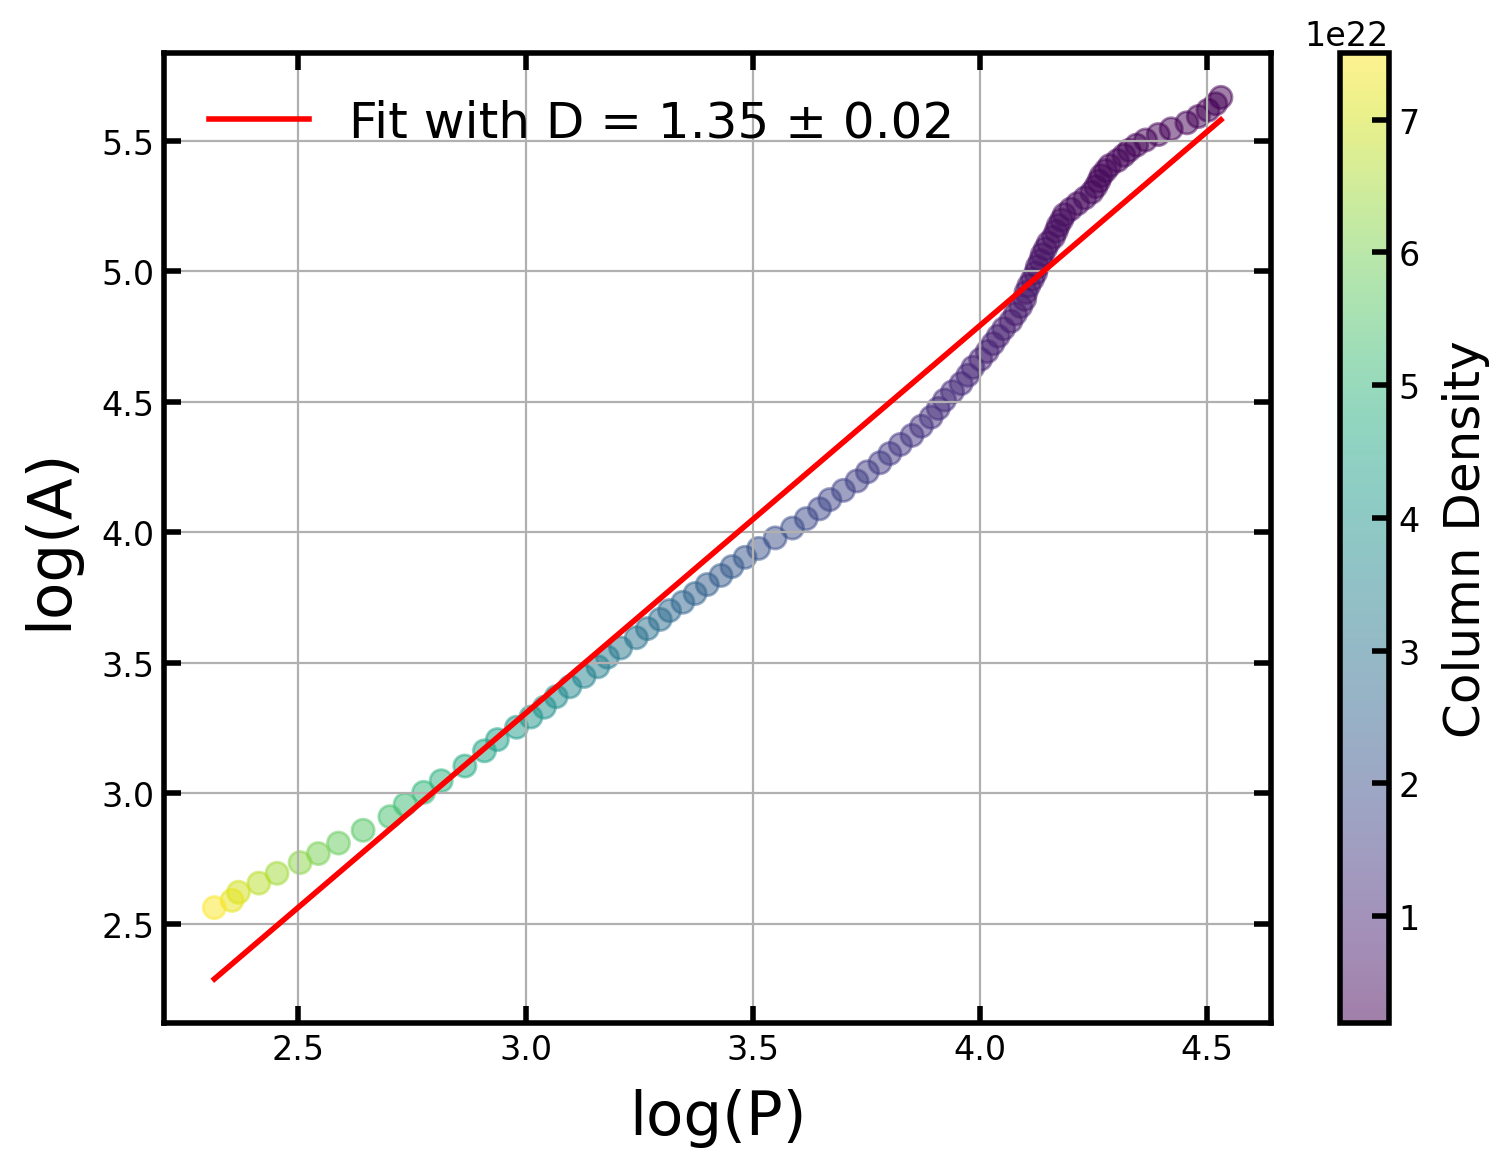
\includegraphics[width=0.5\textwidth]{figures/orion_A_global.png}
    \caption{Perimeter-area relation for Orion A. The line shows the linear fit in log-log space used to estimate the global fractal dimension $D$. Residuals of the fit are shown below the main panel.}
    \label{fig:orion_A_global}
\end{figure}

The Orion A cloud exhibits significant deviations from a single linear fit over the entire column density range. To account for this, a segmented (double) linear fit was applied, splitting the data at $N = 1.23 \times 10^{22}\,\mathrm{cm}^{-2}$. The results of the two fits are:

\begin{equation}
    \notag
    D_1 = 1.65 \pm 0.01 \quad \text{(high column density)}
\end{equation}
\begin{equation}
    \notag
    D_2 = 0.97 \pm 0.02 \quad \text{(low column density)}
\end{equation}

The mean absolute residuals are 0.0222 for the high column density range (correlation coefficient = 0.9986) and 0.0679 for the low column density range (correlation coefficient = 0.9748), indicating an improved agreement with the data compared to the previous single-fit model.

Figure \ref{fig:orion_A_global_double_fit} shows the perimeter-area relation with the two linear fits overlaid and the residuals. The change in slope suggests a structural transition or the presence of different regimes of spatial complexity in the cloud.

\begin{figure}[t]
    \centering
    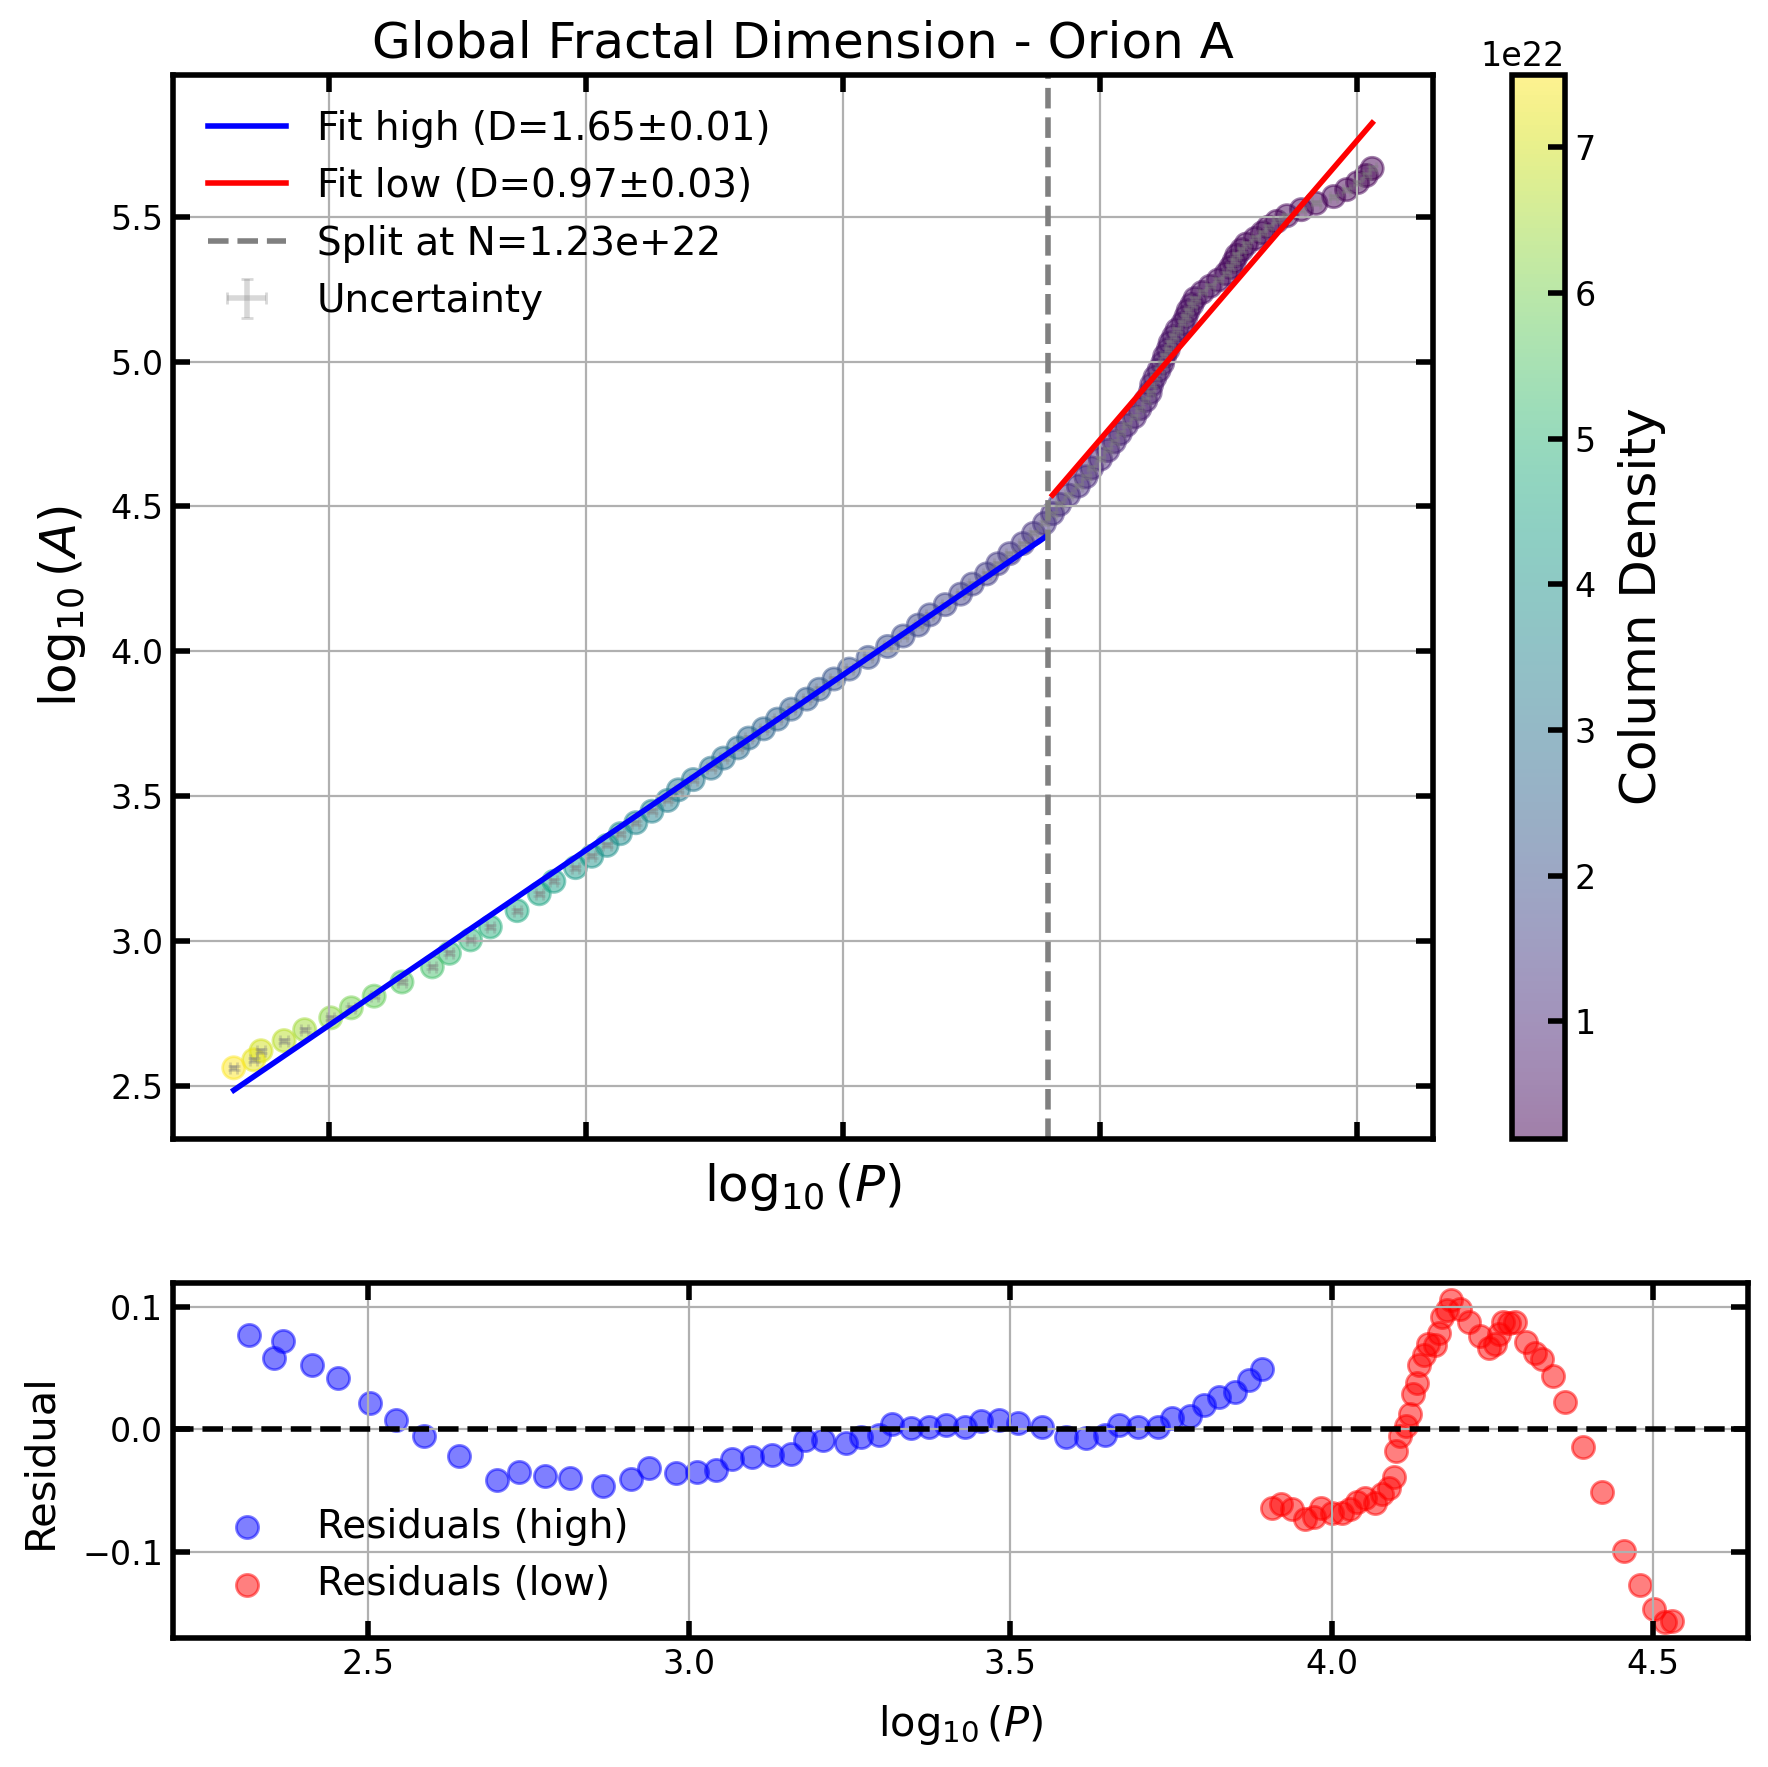
\includegraphics[width=0.5\textwidth]{figures/orion_A_global_double_fit.png}
    \caption{Perimeter-area relation for Orion A with a segmented linear fit. The dashed lines indicate the two fitted regimes, separated at $N=1.23 \times 10^{22}\,\mathrm{cm}^{-2}$. Residuals of the fits are shown below the main panel.}
    \label{fig:orion_A_global_double_fit}
\end{figure}

The Orion B cloud exhibits a well-behaved perimeter-area relation that can be accurately described by a single linear fit across the entire column density range. The results are:

\begin{equation}
    \notag
    D_{\mathrm{OB,\,Global}} = 1.40 \pm 0.01
\end{equation}

Figure \ref{fig:orion_B_global} shows the perimeter-area relation together with the fitted line and residuals. The consistency of the slope across scales suggests a more uniform structural complexity compared to Orion A. The mean absolute residual is $0.0493$ and the correlation coefficient $0.9976$.

\begin{figure}[t]
    \centering
    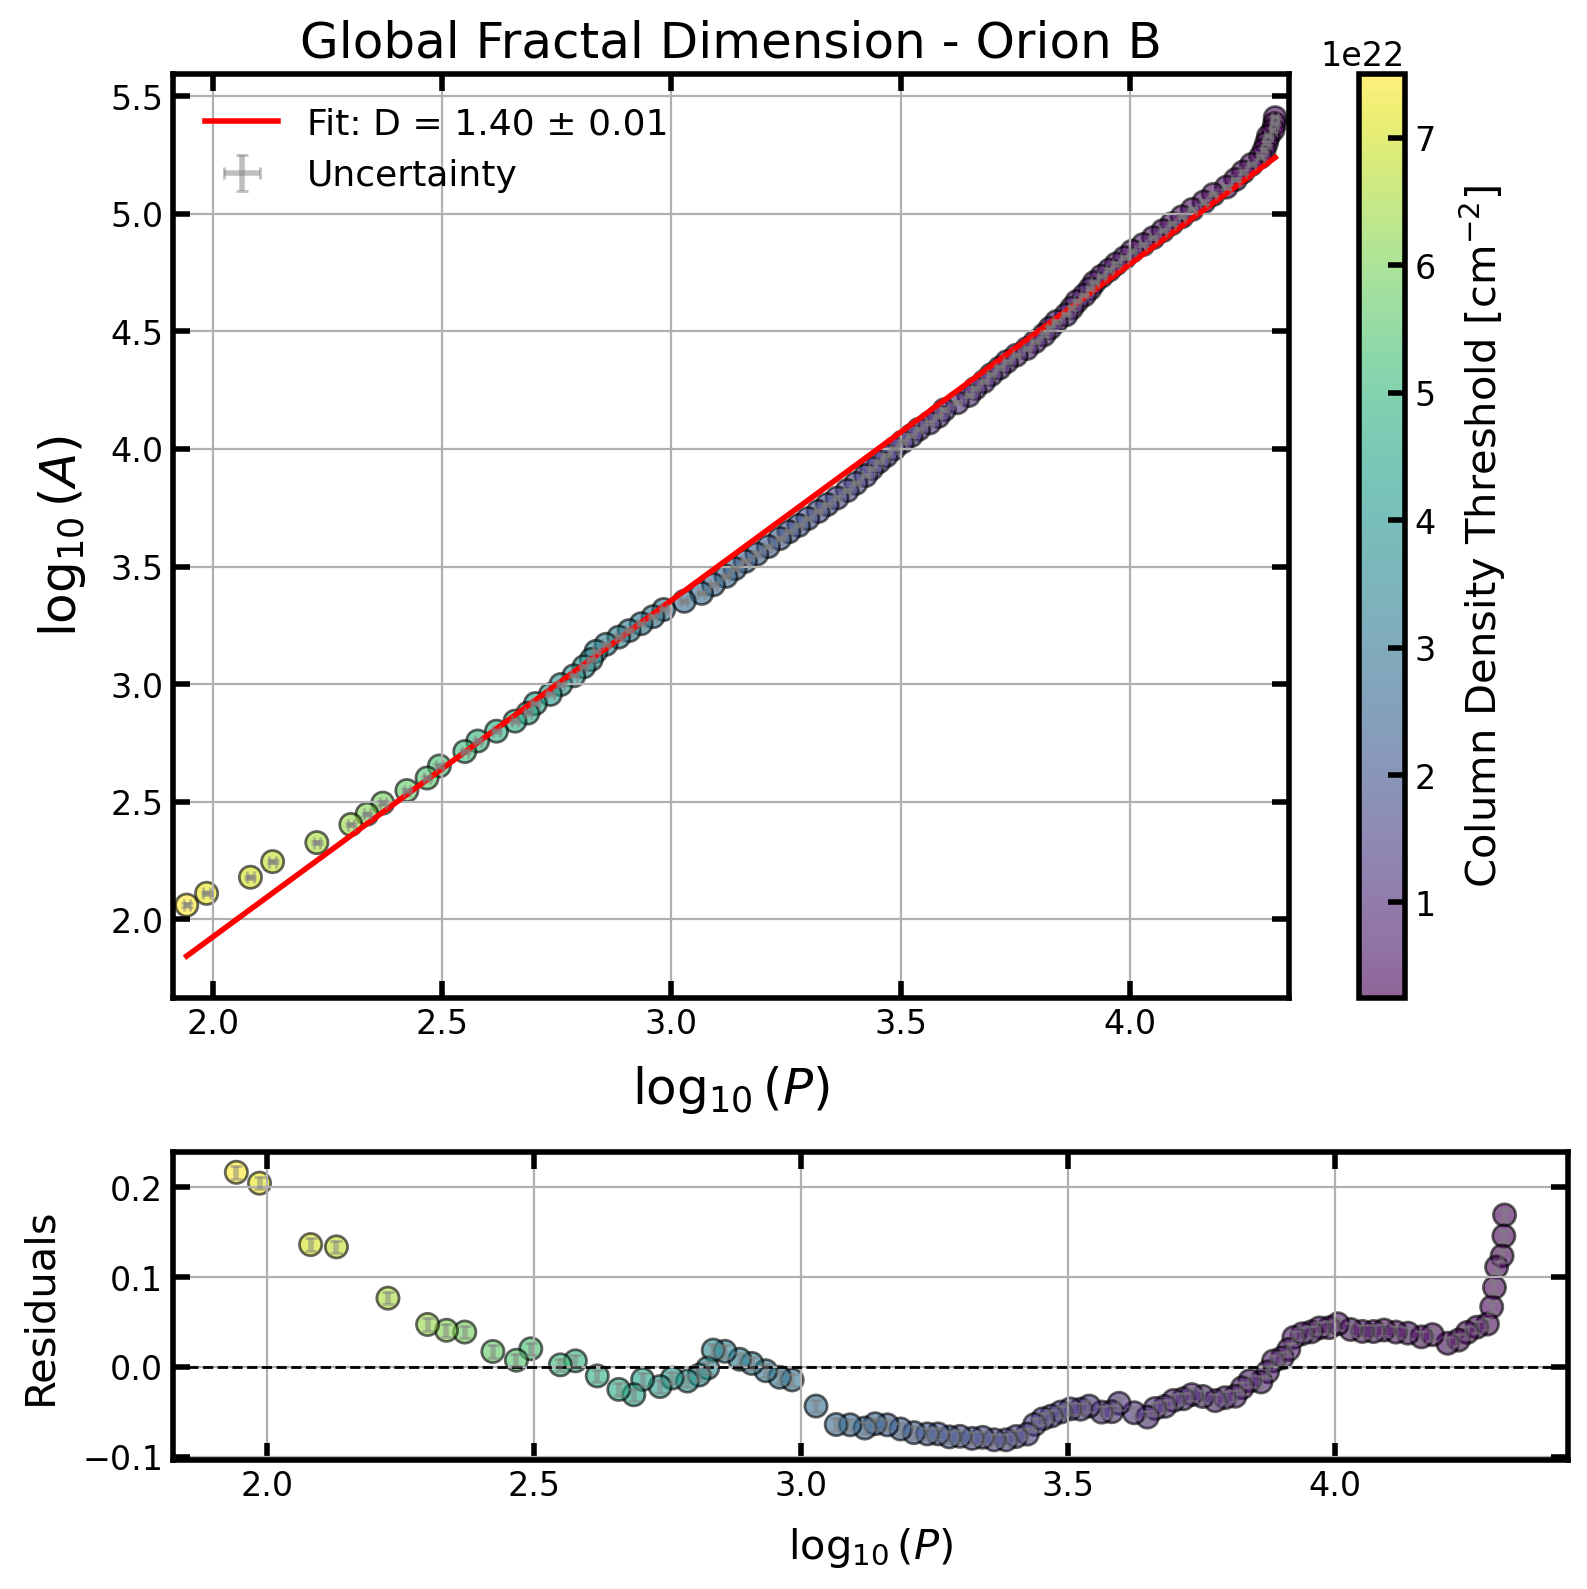
\includegraphics[width=0.5\textwidth]{figures/orion_B_global.png}
    \caption{Perimeter-area relation for Orion B with the best-fit linear regression overlaid. Residuals of the fit are shown below the main panel.}
    \label{fig:orion_B_global}
\end{figure}

The uncertainties in perimeter and area were estimated as 1.6\% from simulation results, which demonstrated that this level of error is representative across different reference geometries.

% To-Do:
% Explicitly say the N_min and N_max
\section{Local Properties}

\subsection{Euler Characteristic}

We computed the Euler characteristic for both Orion A and Orion B, as presented in Figures \ref{fig:Euler_Orion_A_no_figs} and \ref{fig:Euler_Orion_B_no_figs}. This topological descriptor provides insight into the degree of connectivity and fragmentation within the molecular clouds.

\begin{figure}[t]
    \centering
    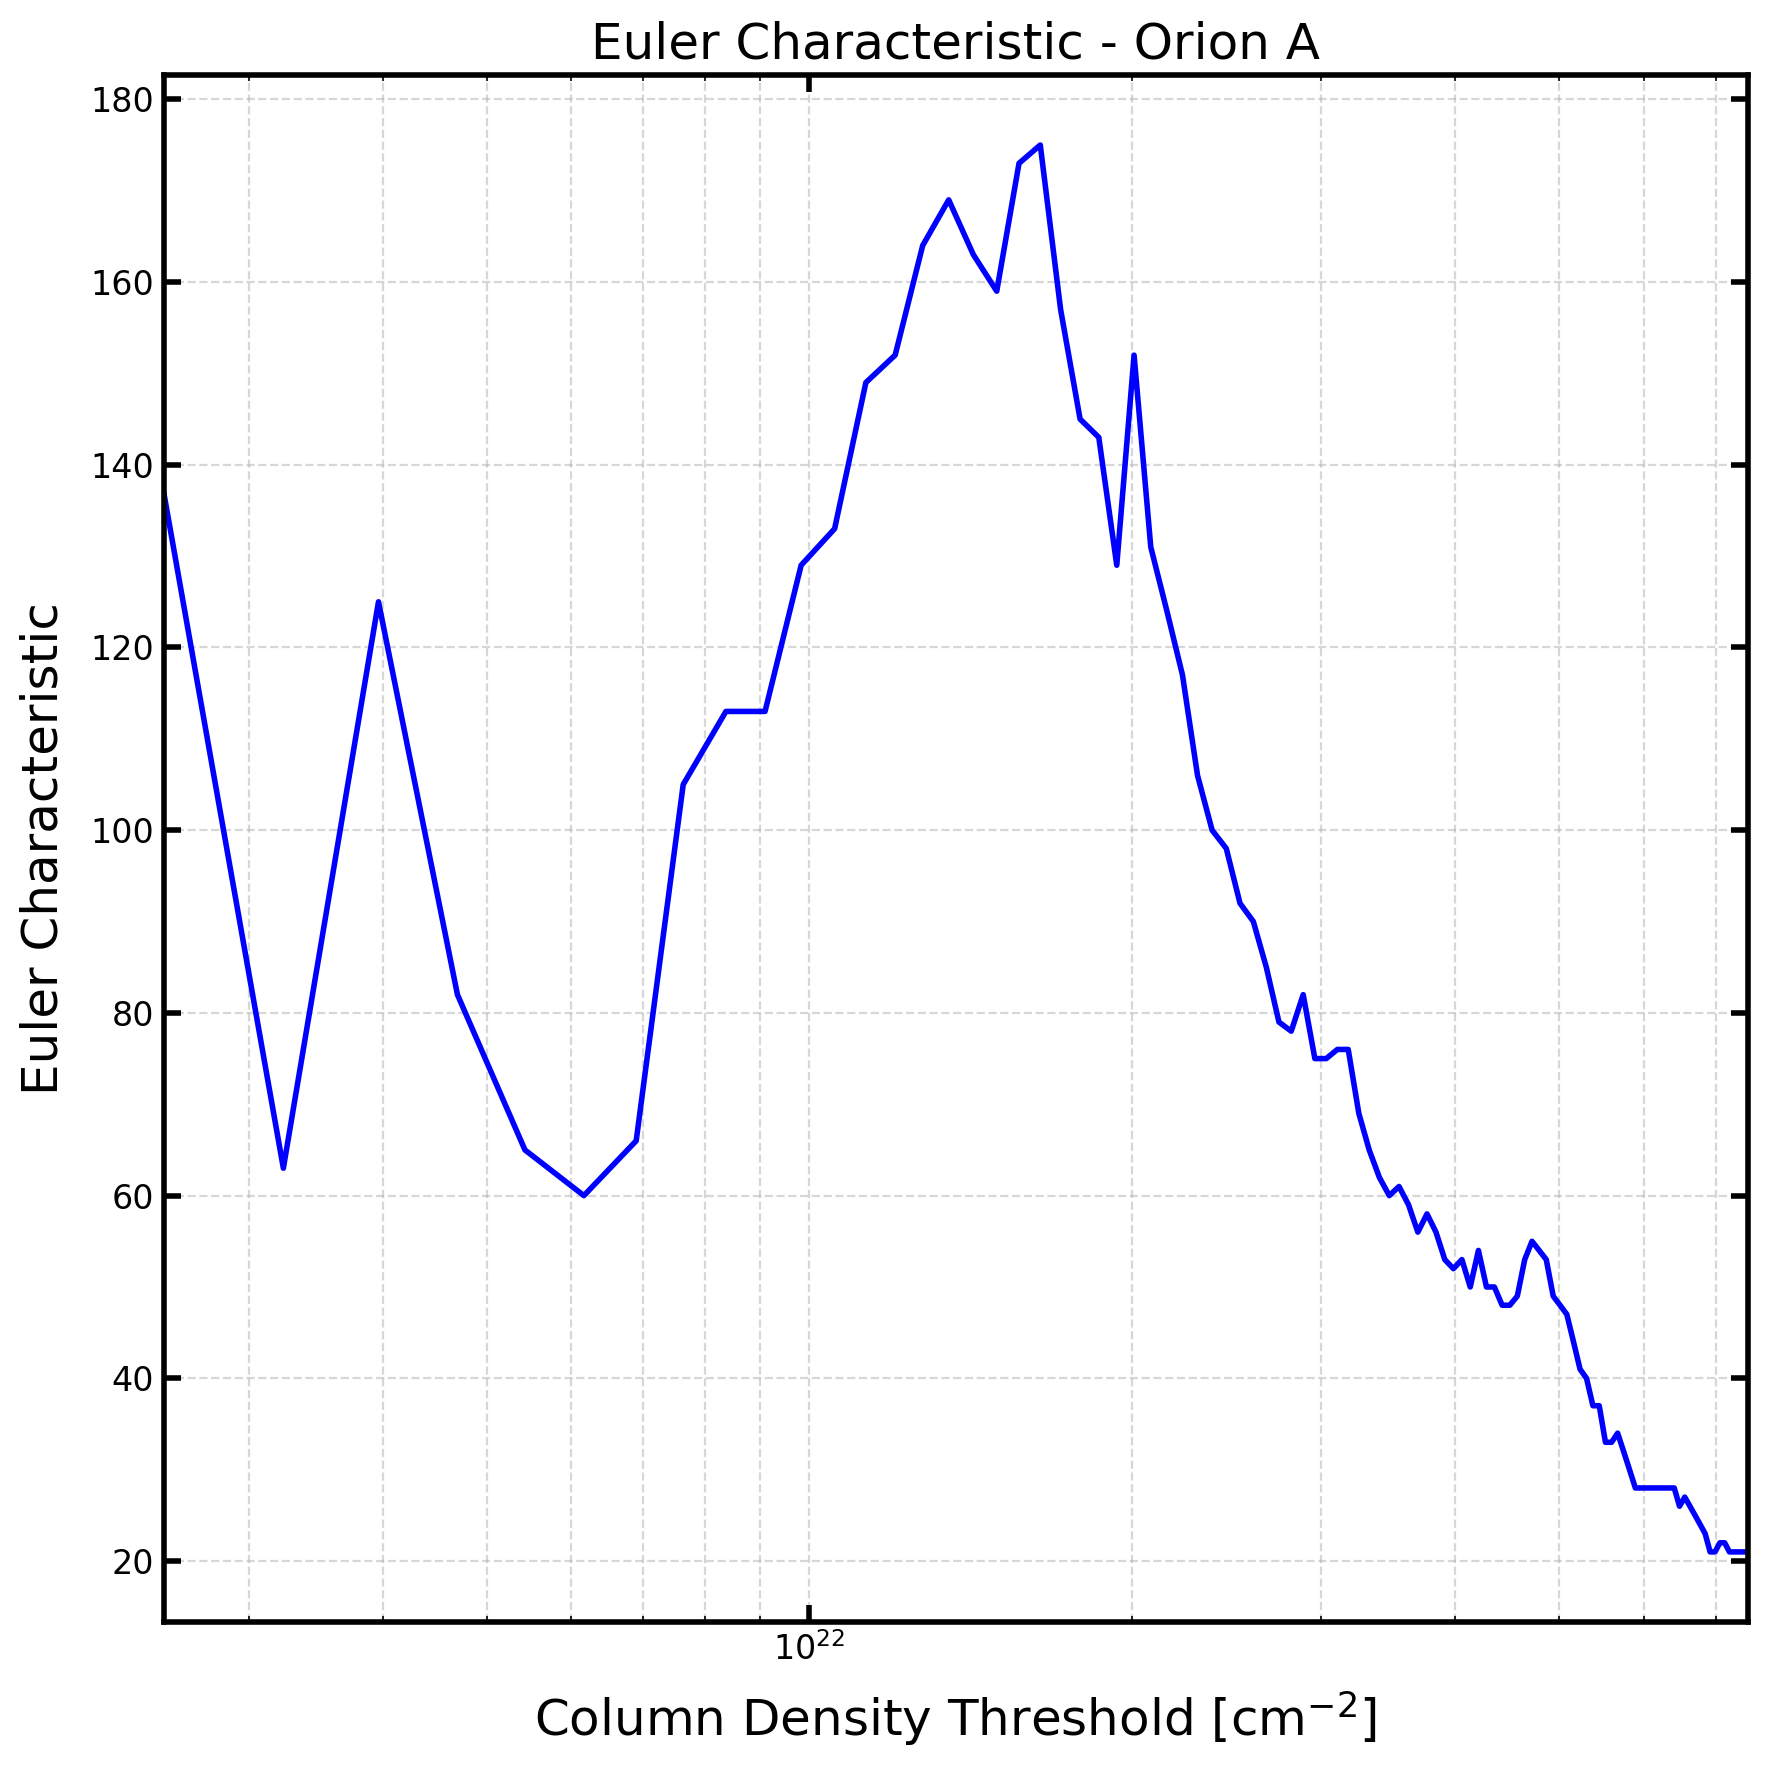
\includegraphics[width=0.5\textwidth]{figures/euler_Orion_A_no_figs.png}
    \caption{Euler characteristic of Orion A as a function of column density threshold.}
    \label{fig:Euler_Orion_A_no_figs}
\end{figure}

\begin{figure}[t]
    \centering
    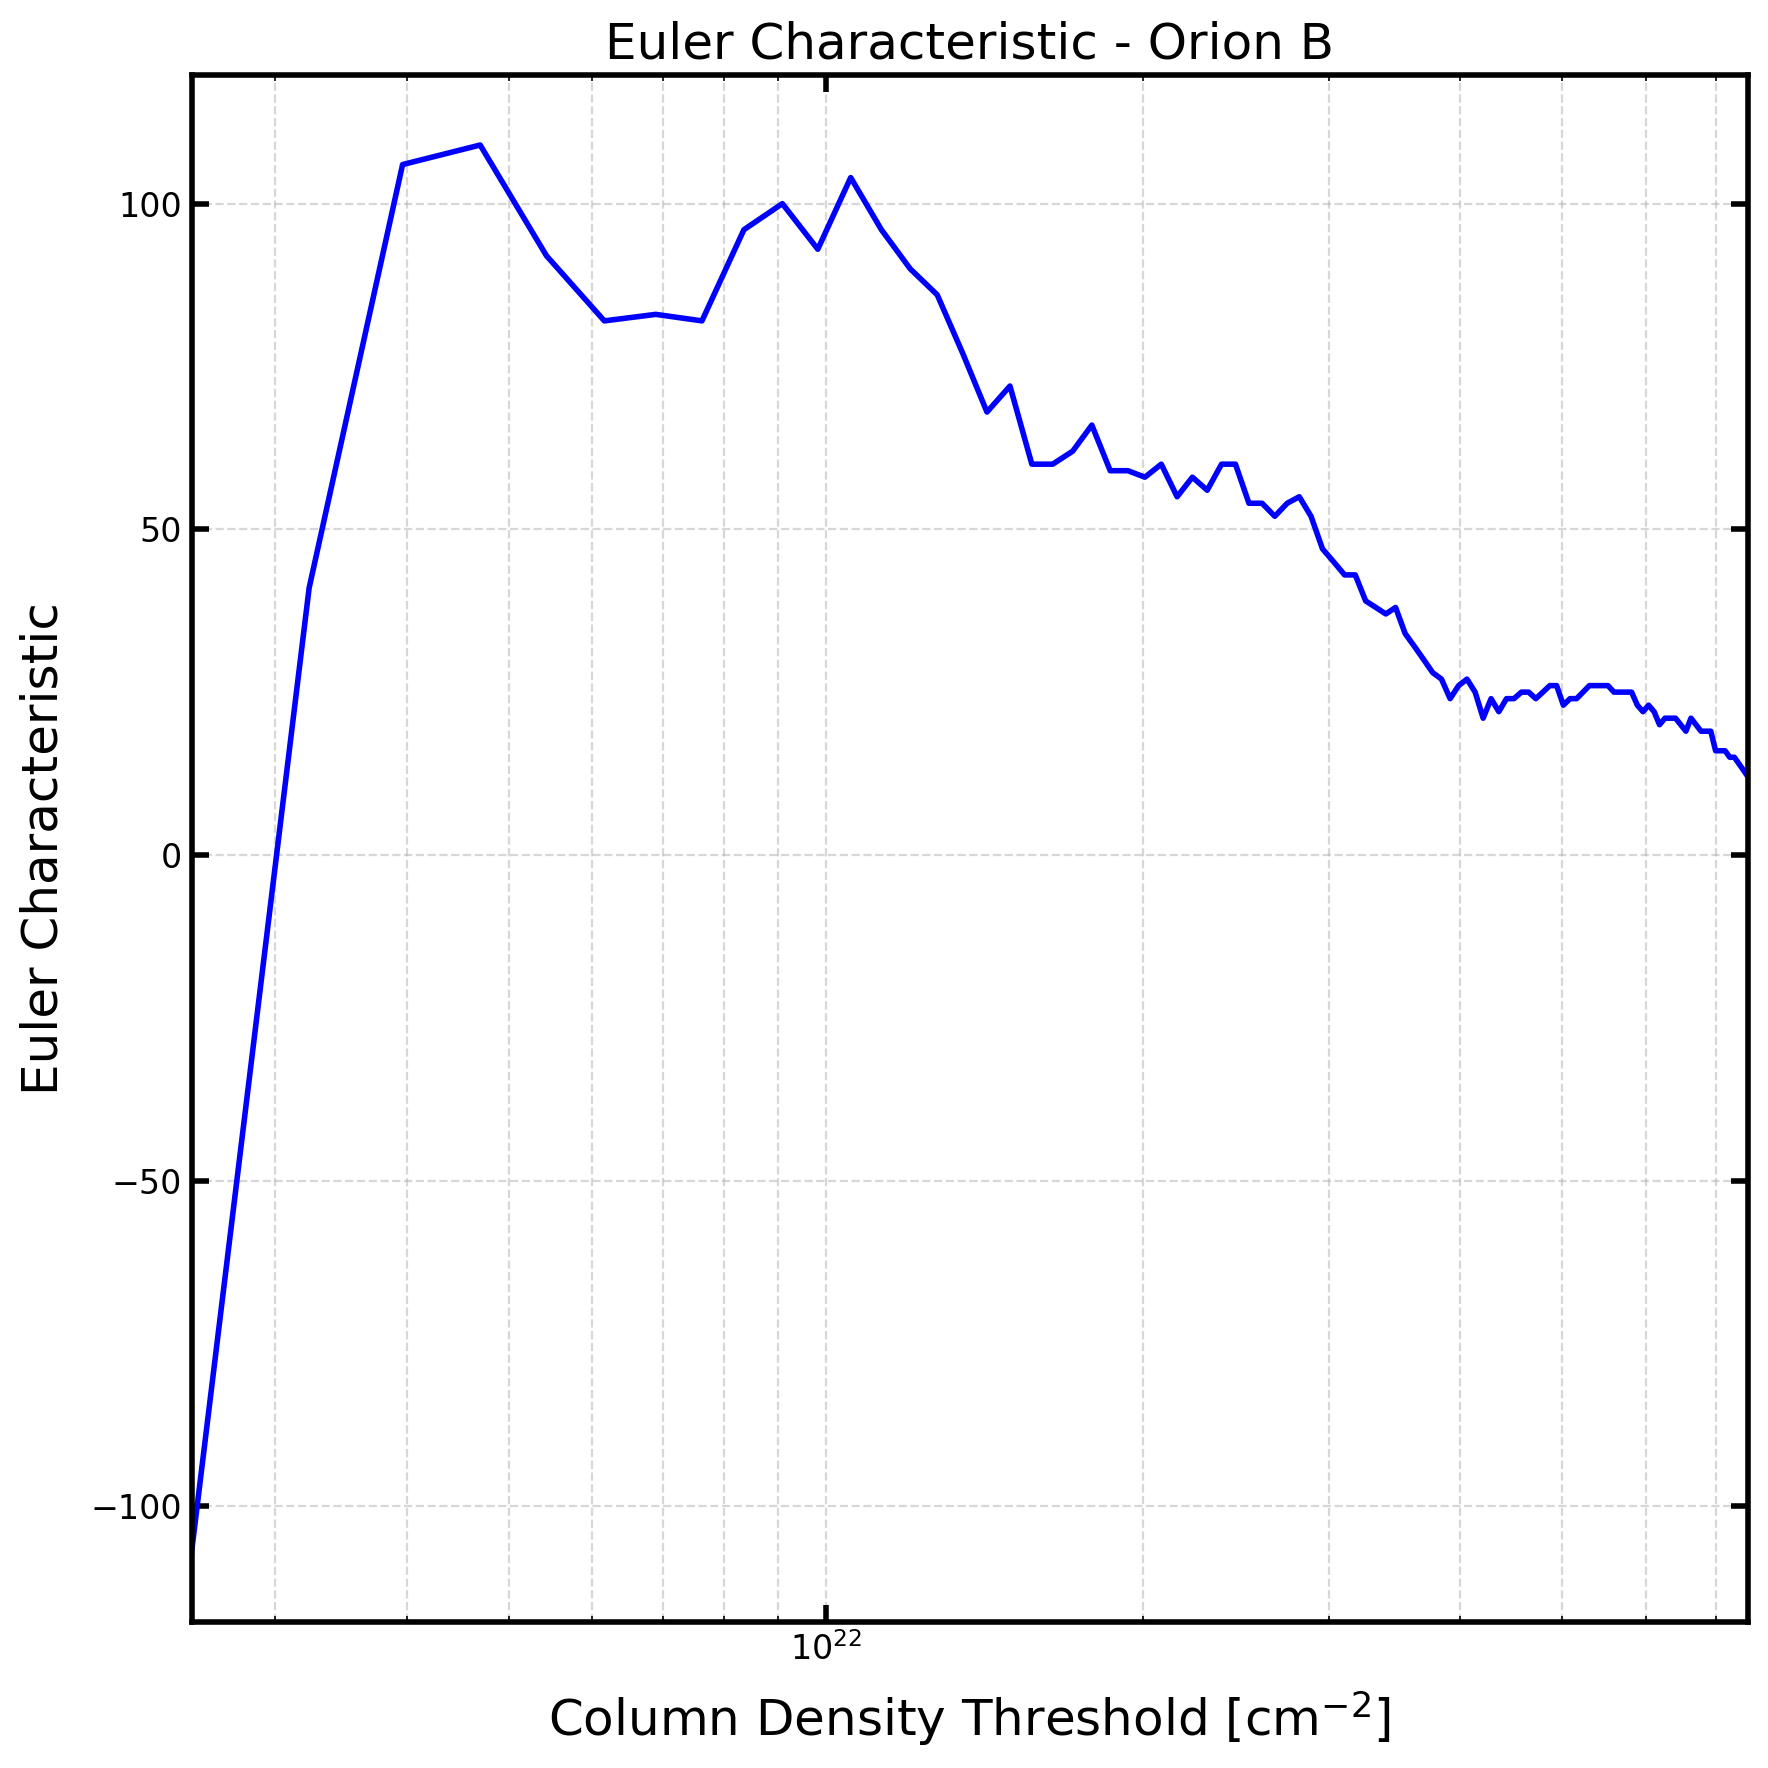
\includegraphics[width=0.5\textwidth]{figures/euler_Orion_B_no_figs.png}
    \caption{Euler characteristic of Orion B as a function of column density threshold.}
    \label{fig:Euler_Orion_B_no_figs}
\end{figure}

\subsection{Local Fractal Dimension}

The data for the local fractal dimension as a function of column density threshold for Orion A and Orion B are presented in Figure~\ref{fig:local_Orion_A_B}. Both regions show a clear overall trend in which the local fractal dimension varies systematically with increasing threshold. Notably, several pronounced peaks and deviations from the trend are observed. These features may correspond to transitions in the morphology of the structures, such as the emergence or fragmentation of dense cores and filaments.  

A more detailed analysis of the origins of these peaks and their significance in the context of cloud evolution and turbulence will be carried out in the subsequent sections. In particular, it will be important to assess whether these variations reflect genuine changes in the underlying structure or are influenced by resolution limits and noise at higher thresholds.

\begin{figure}[t]
    \centering
    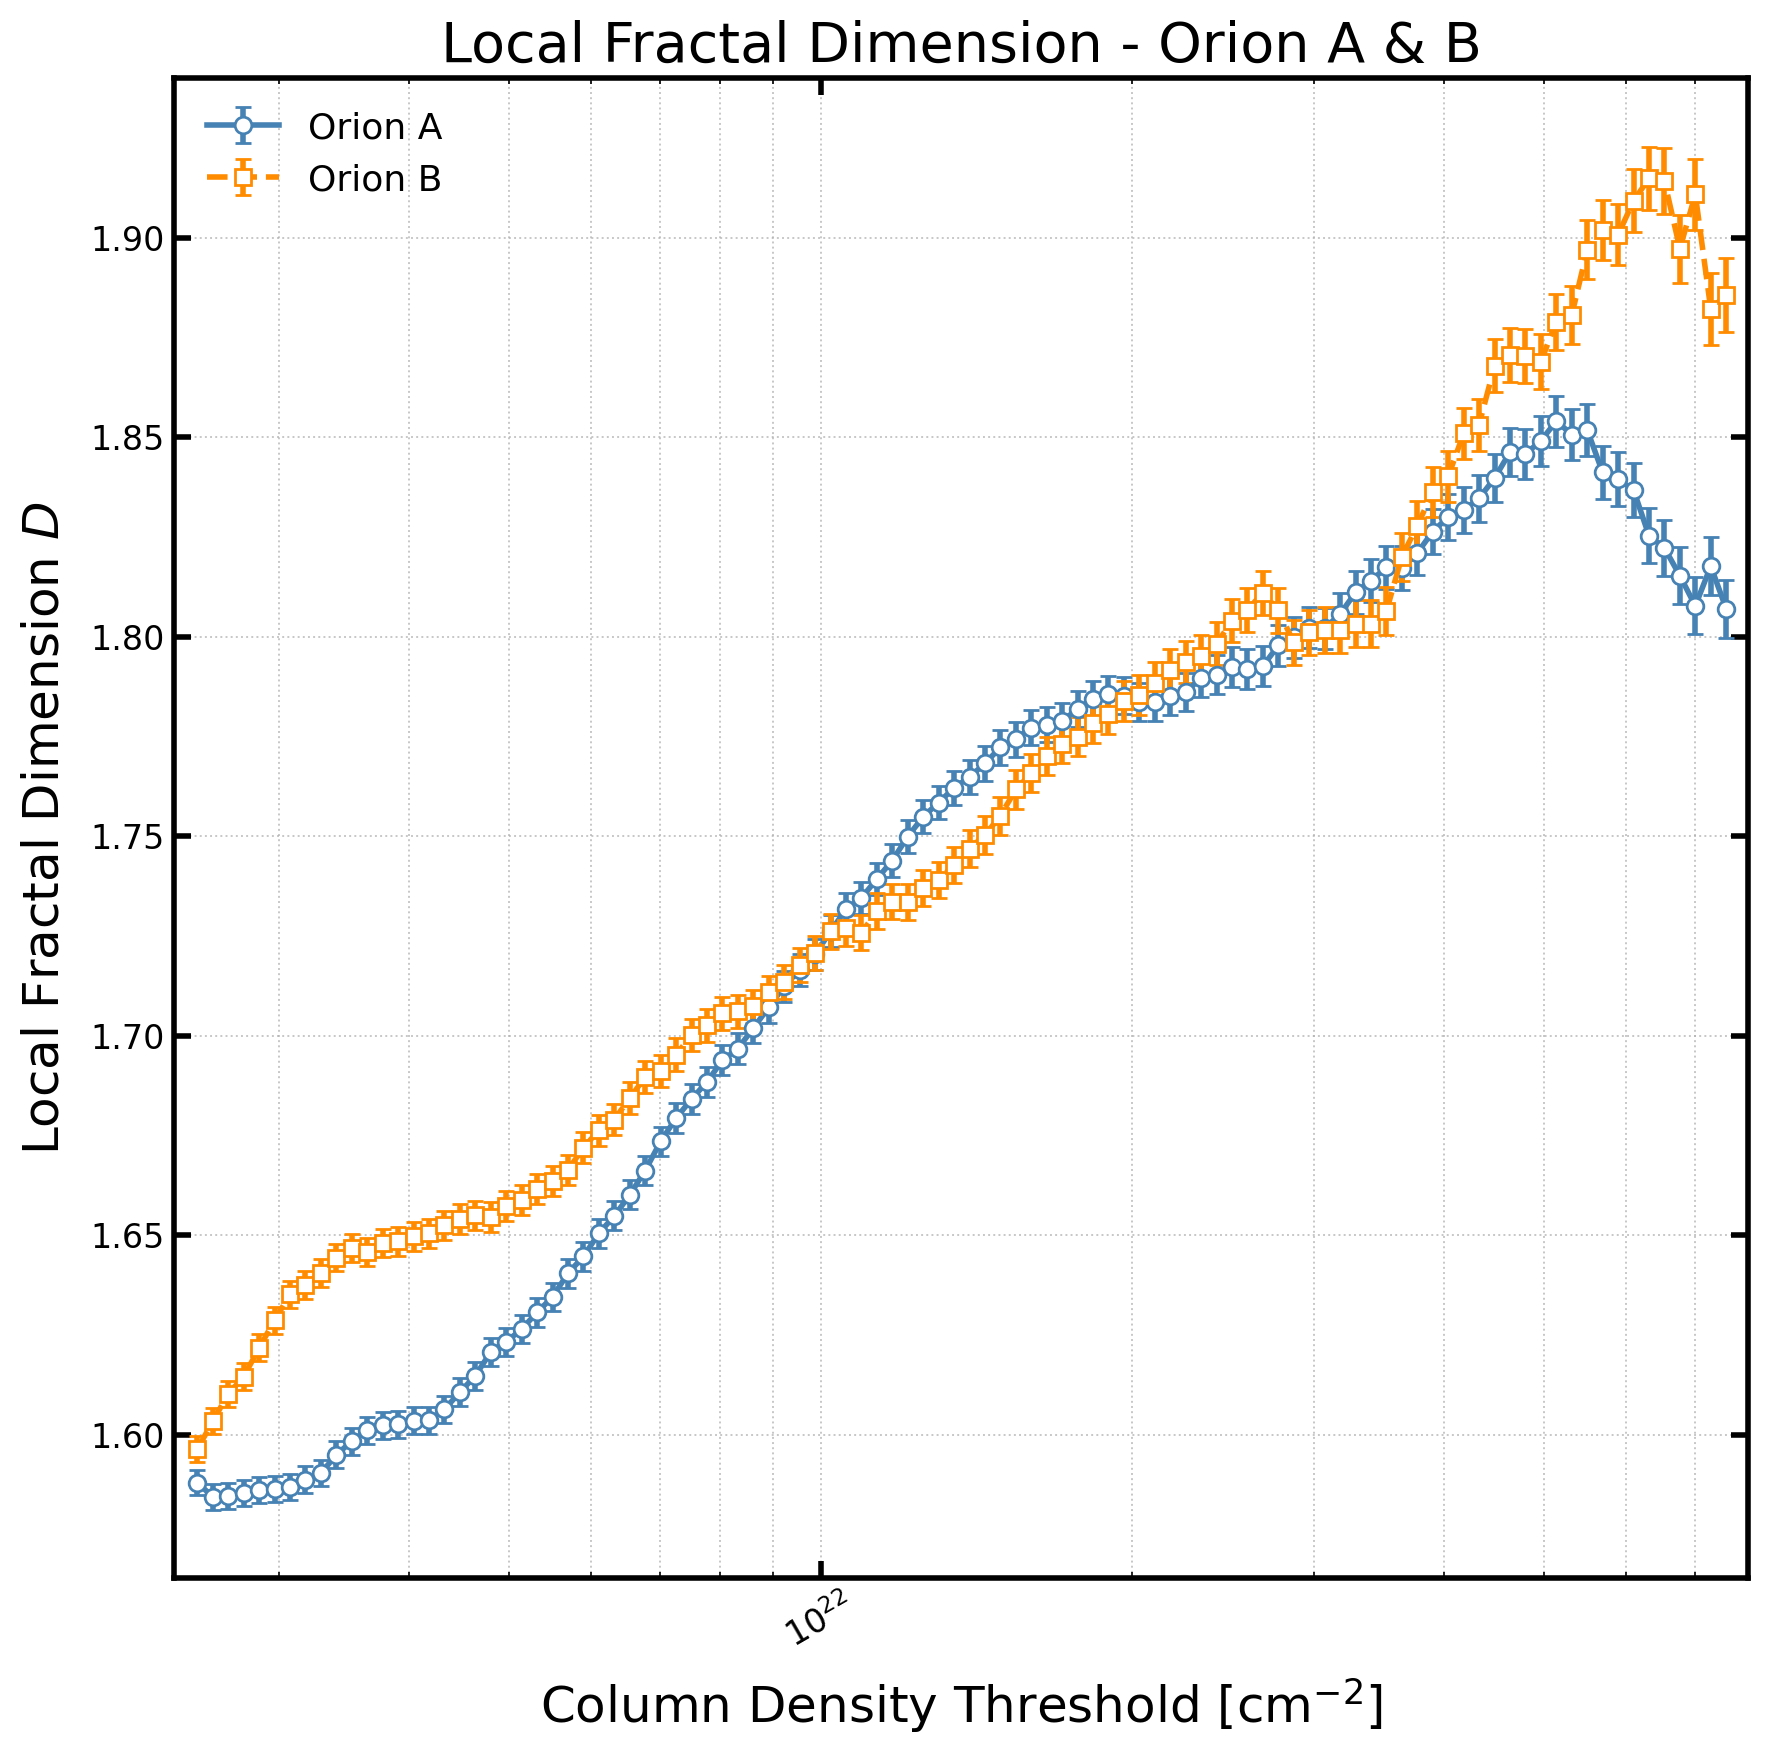
\includegraphics[width=0.6\textwidth]{figures/local_orion_A_B.png}
    \caption{Local fractal dimension as a function of column density threshold for Orion A and Orion B, including the corresponding uncertainties.}
    \label{fig:local_Orion_A_B}
\end{figure}

\subsection{Analysis of Individual Structures}

To gain deeper insight into the fractal properties of the cloud, we subdivided each column density threshold into the set of connected structures that emerge at that threshold level. This dendrogram-based approach provides a hierarchical perspective on how the material organizes into nested substructures, enabling a more detailed examination of their characteristics.

Figures \ref{fig:dendrogram_A} and \ref{fig:dendrogram_B} show the resulting dendrograms for Orion A and Orion B, respectively. These diagrams illustrate how individual regions merge into larger complexes as the threshold decreases, effectively capturing the clustering behaviour of the cloud across scales.

\begin{figure}[t]
    \centering
    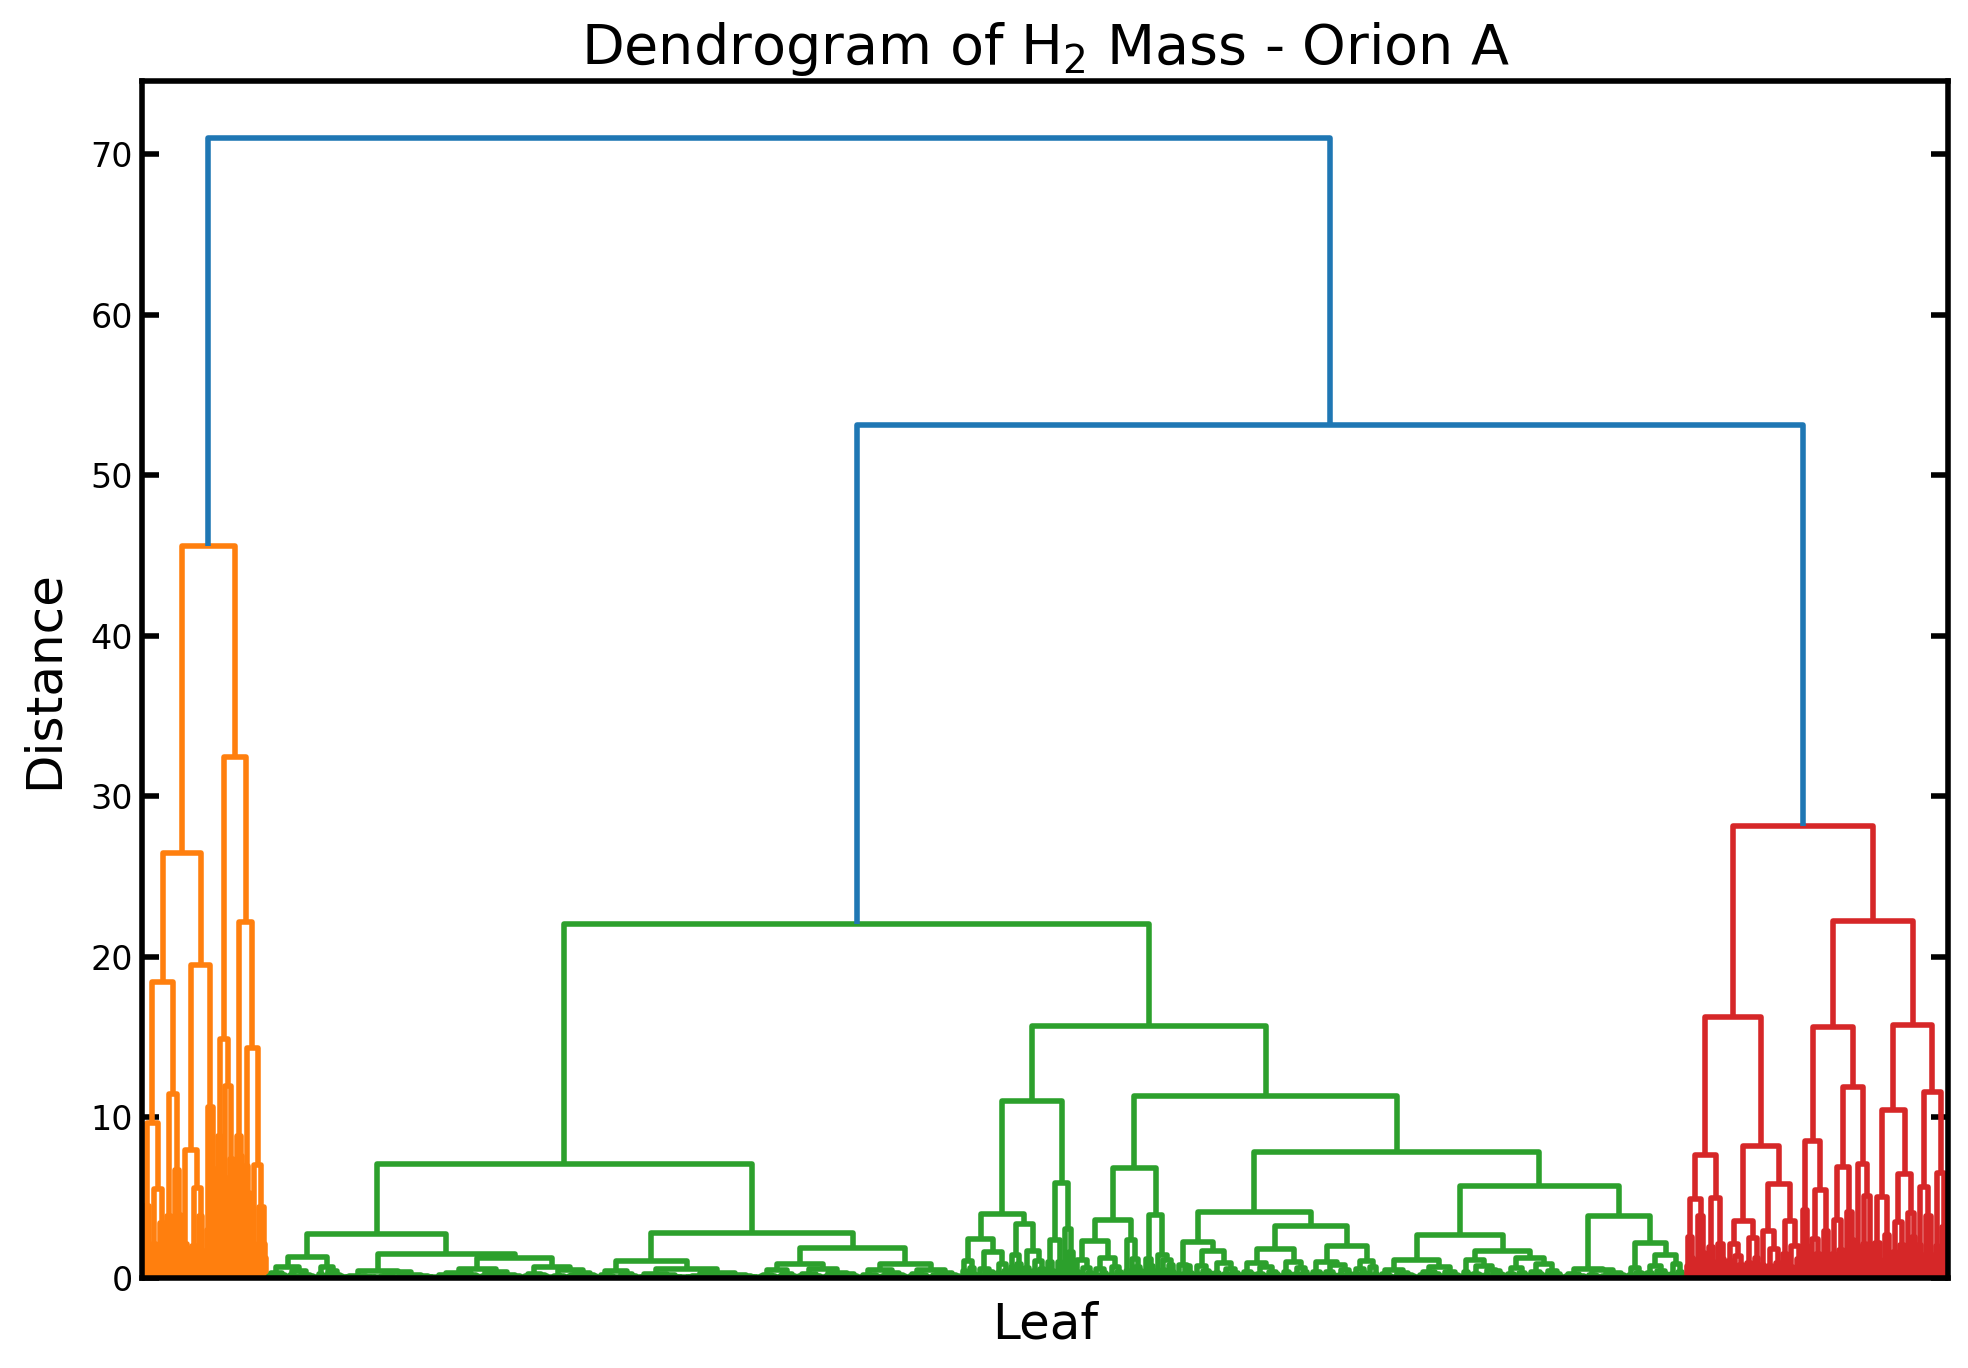
\includegraphics[width=0.6\textwidth]{figures/dendogram_A.png}
    \caption{Dendrogram of the Orion A mass distribution, showing the hierarchical merging of structures as the column density threshold varies.}
    \label{fig:dendrogram_A}
\end{figure}

\begin{figure}[t]
    \centering
    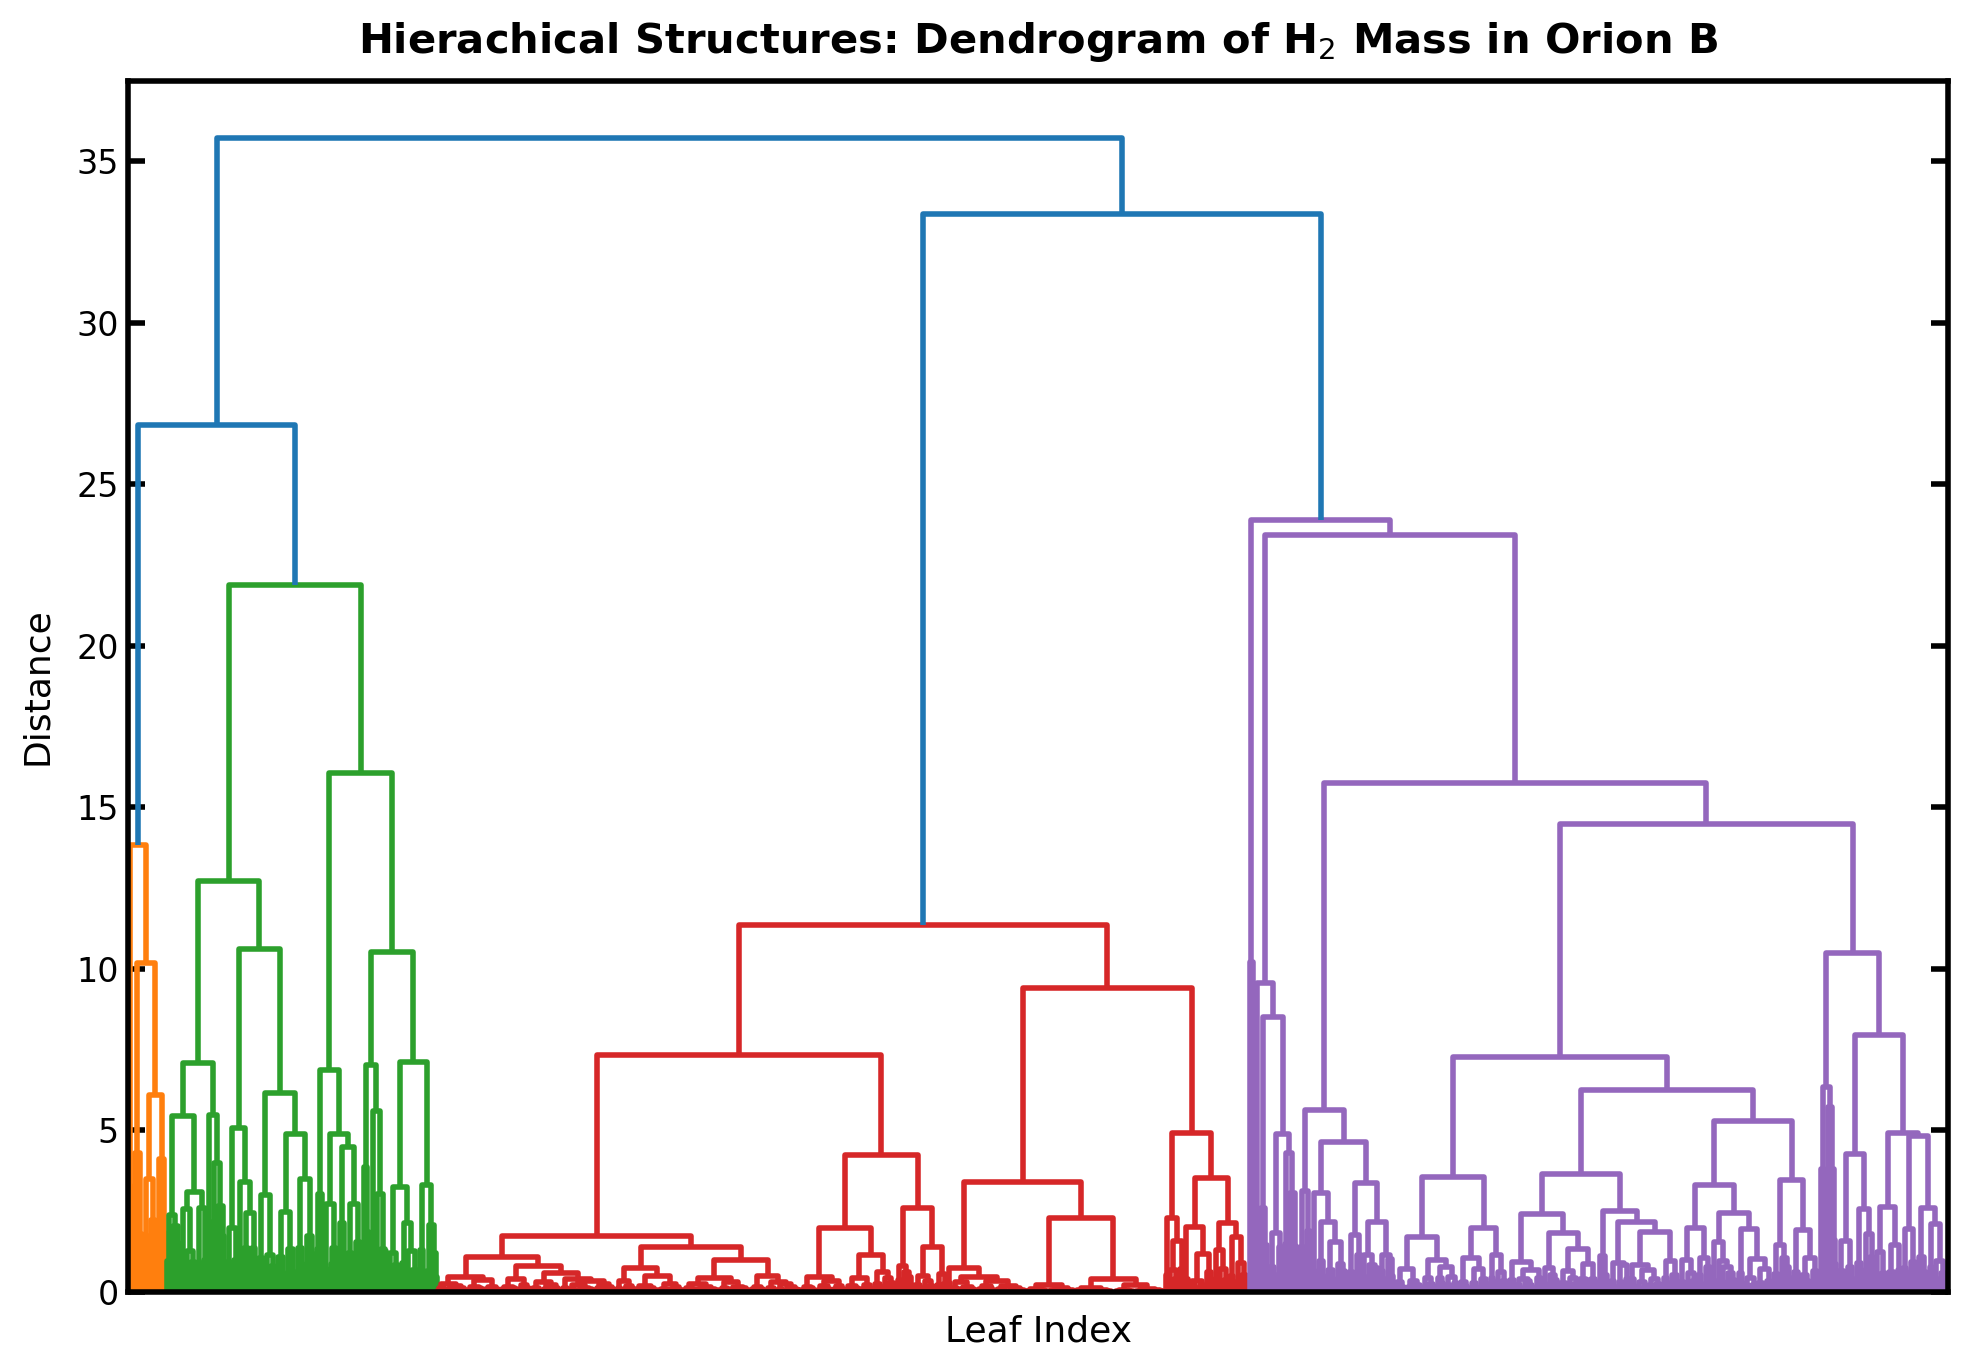
\includegraphics[width=0.6\textwidth]{figures/dendogram_B.png}
    \caption{Dendrogram of the Orion B mass distribution, showing the hierarchical merging of structures as the column density threshold varies.}
    \label{fig:dendrogram_B}
\end{figure}

To further explore the fractal properties at each column density threshold, we extracted the connected structures and applied the same calculation for the local fractal dimension to these.
We divided the calculation at each threshold for a number of biggest regions, satisfying a number of criteria based on pixel perimeter and area to not encounter any numerical error.
The results of these can be seen in Figures \ref{fig:local_A_single_structures} and \ref{fig:local_B_single_structures}, where we recorded similar, but shallower trendds as in the undifferenciated calculation at each threshold (Figure~\ref{fig:local_Orion_A_B}).

% To-Do:
% add errors
% make more similar to local Orion A and B
\begin{figure}[t]
    \centering
    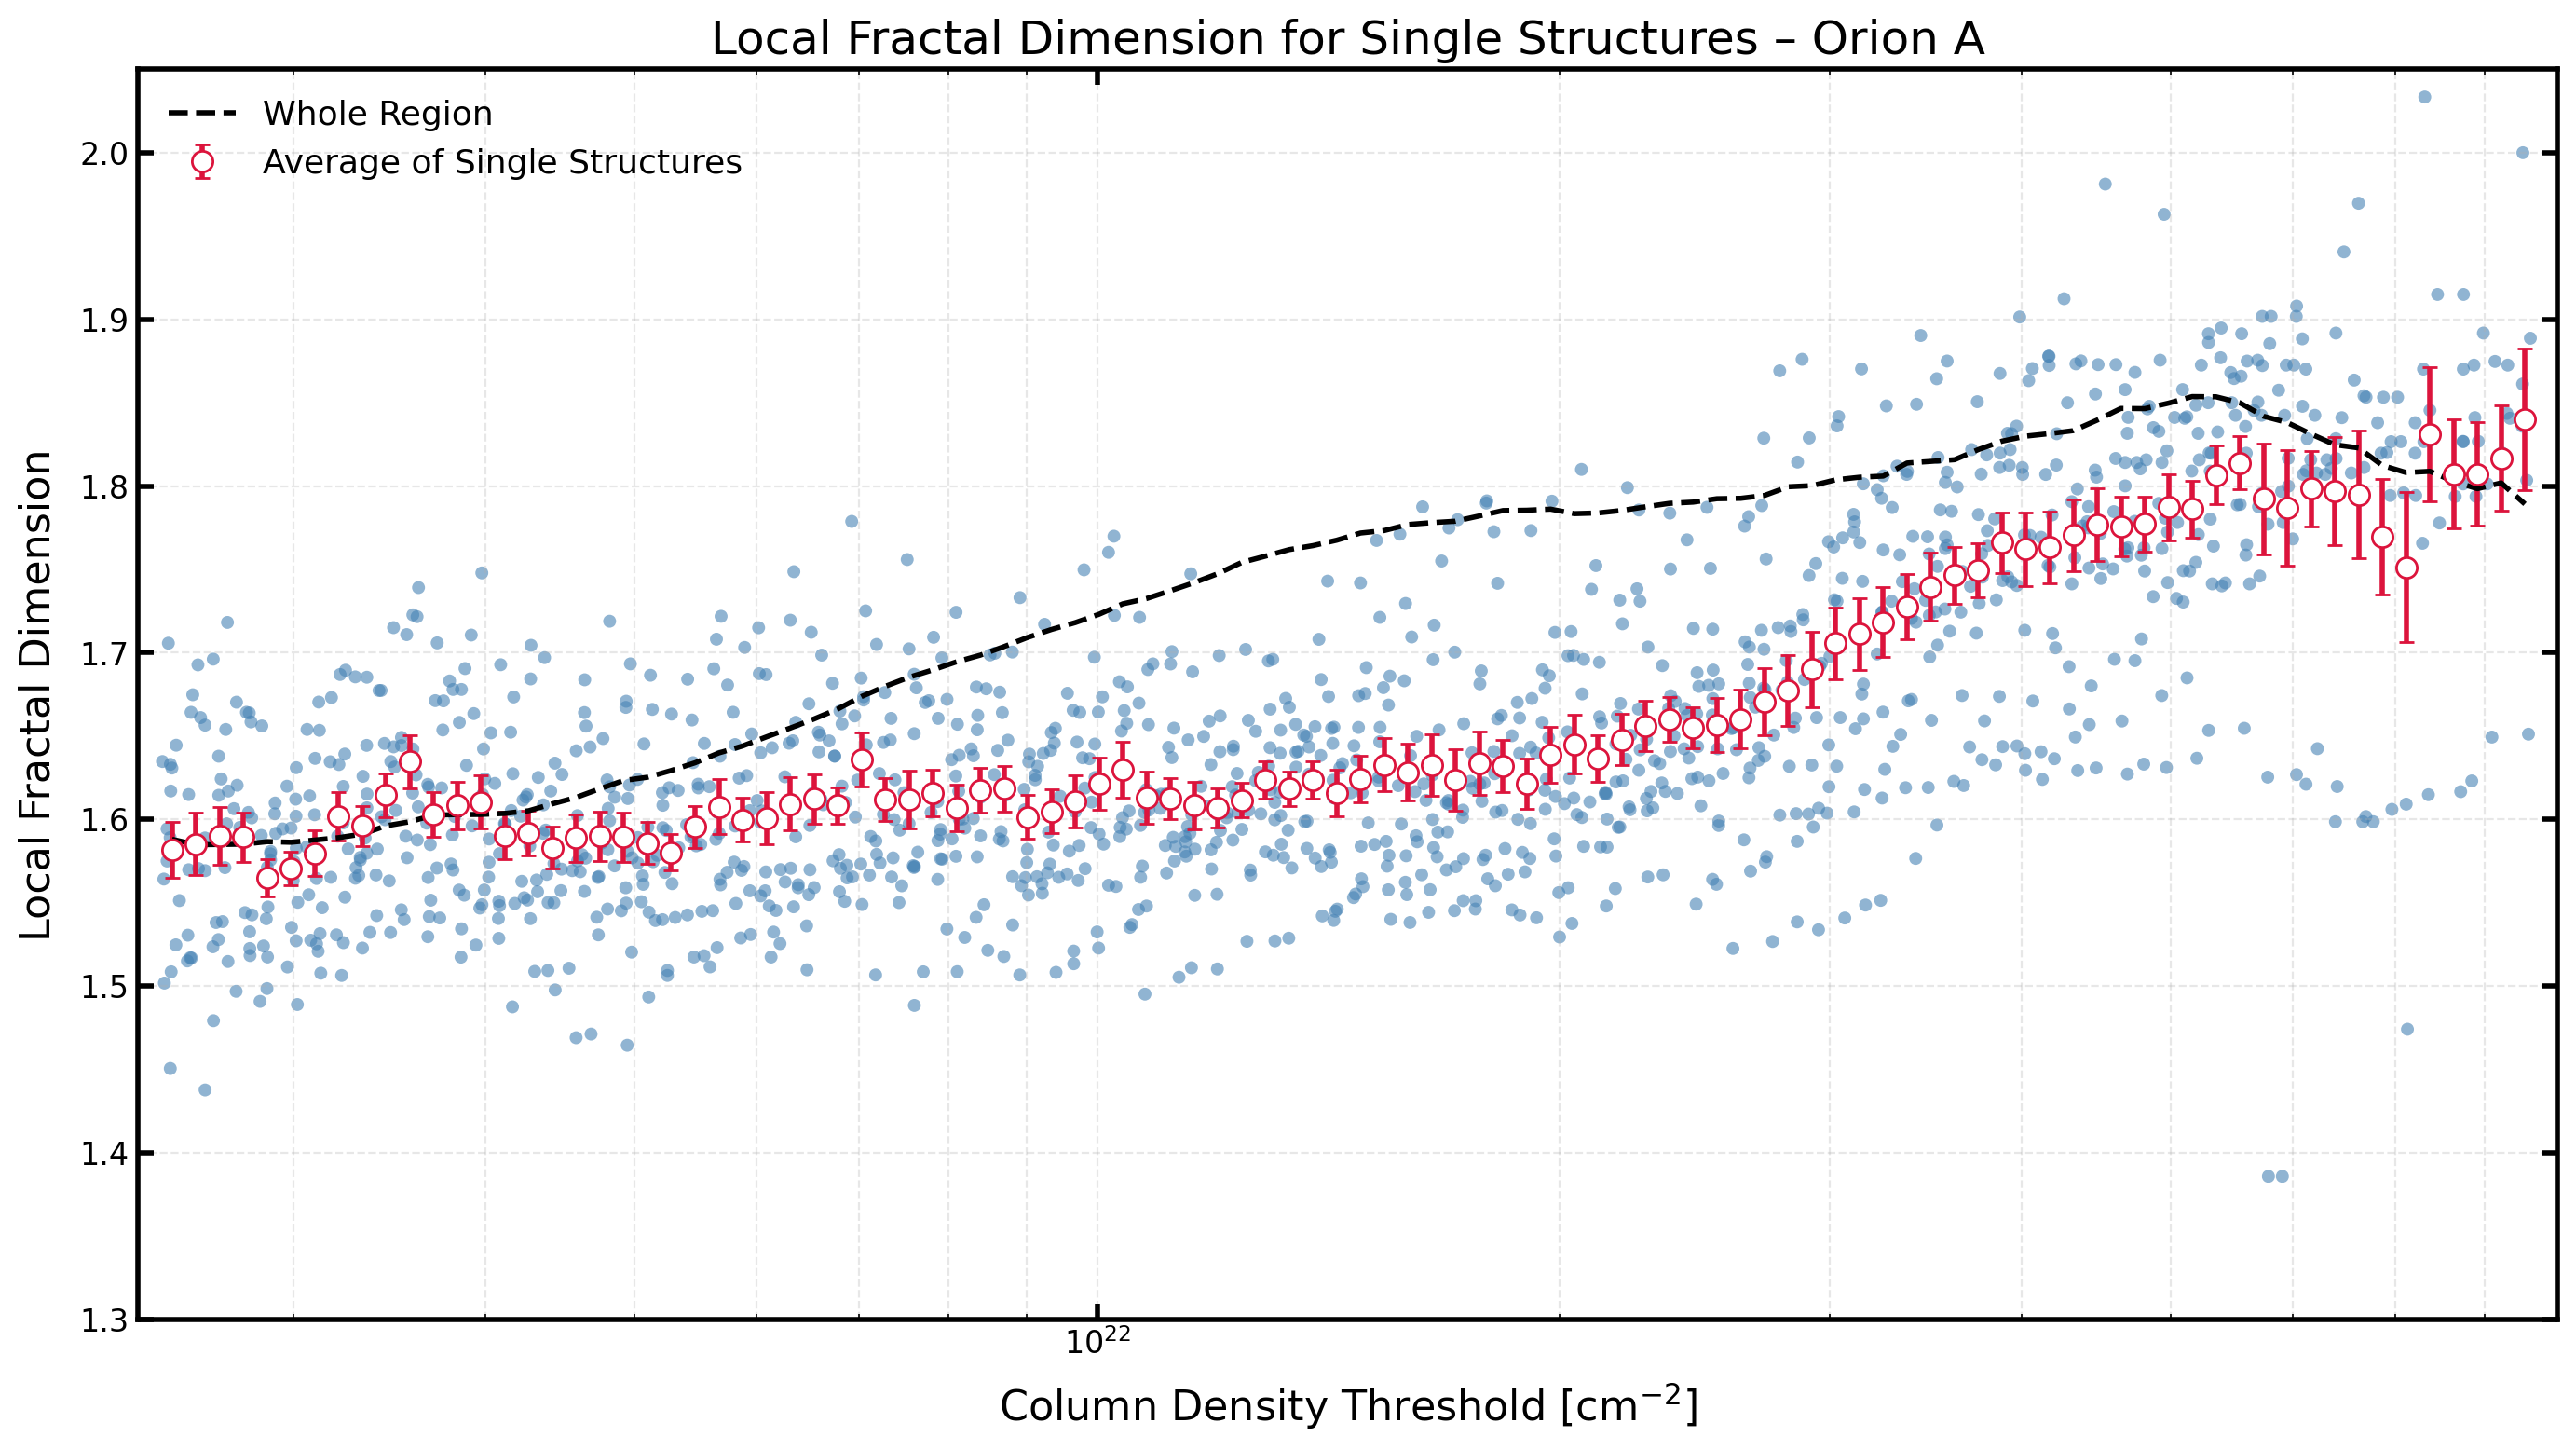
\includegraphics[width=0.7\textwidth]{figures/local_Orion_A_single_structures.png}
    \caption{Local fractal dimension for single structures at each column density threshold for Orion A. Overlaid are both the average of the single regions for each column density threshold as well as the values for the undifferncited calculation. Uncertainties are included.}
    \label{fig:local_A_single_structures}
\end{figure}

\begin{figure}[t]
    \centering
    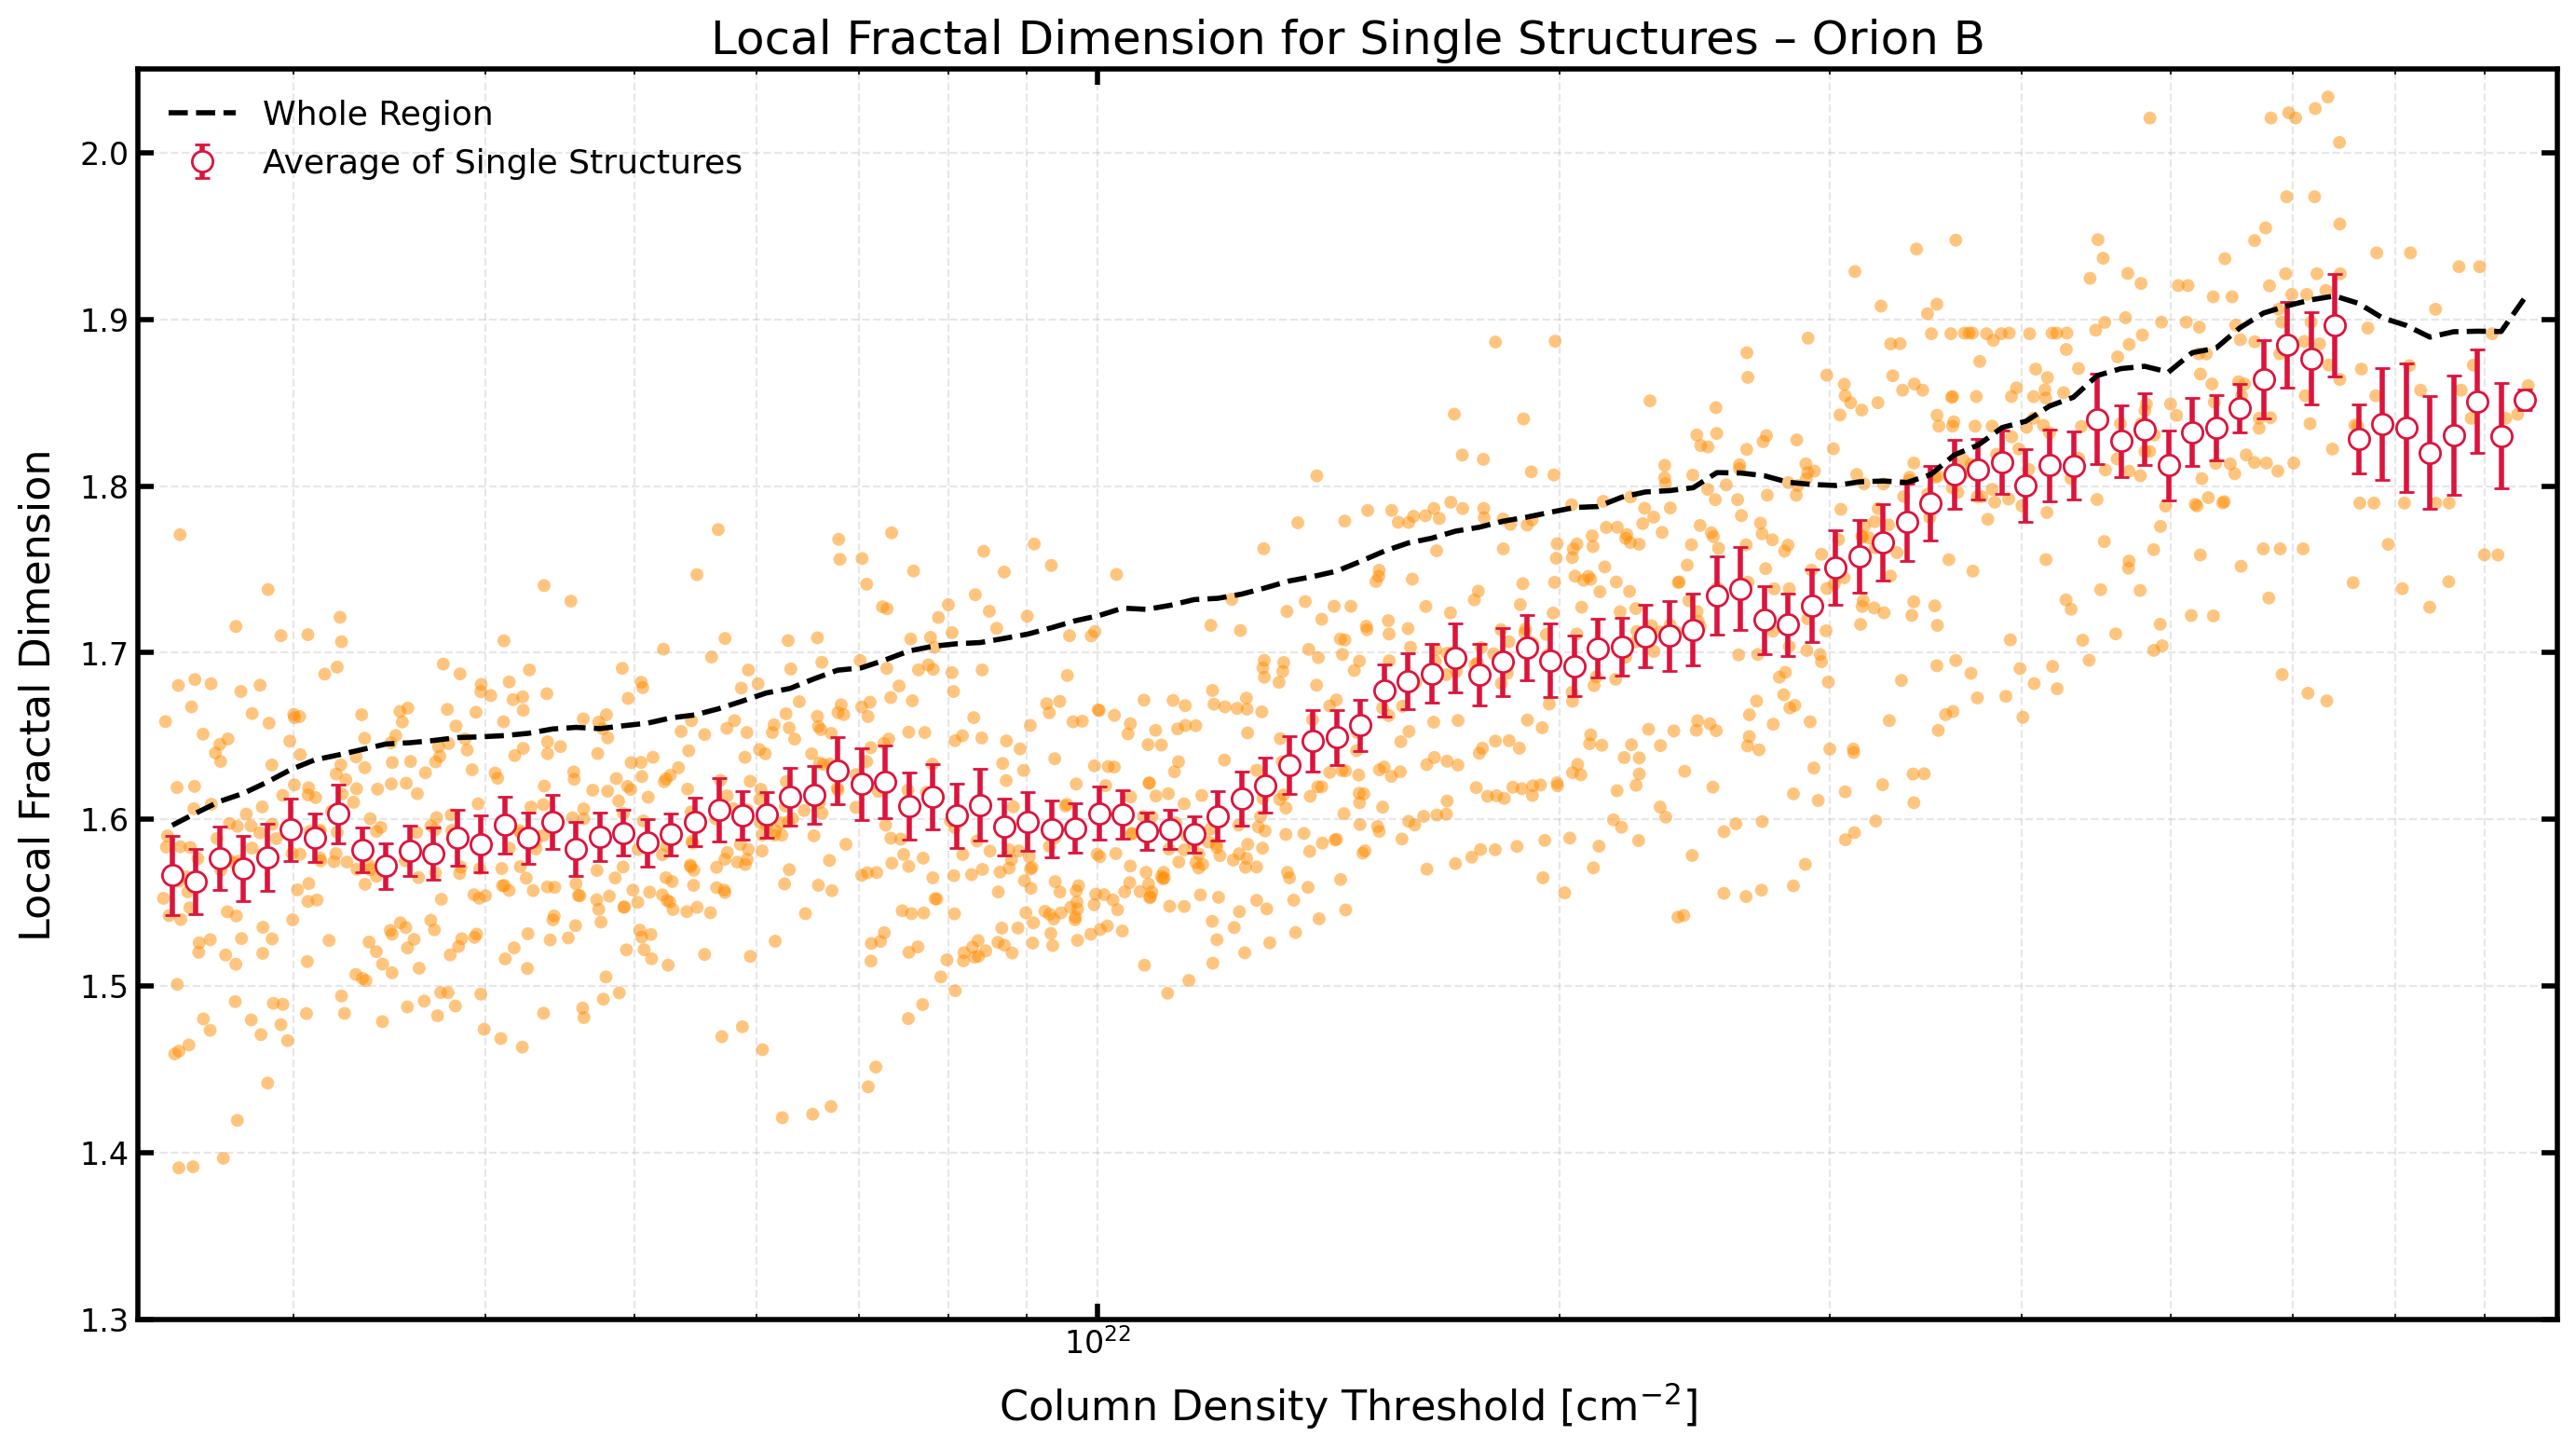
\includegraphics[width=0.7\textwidth]{figures/local_Orion_B_single_structures.png}
    \caption{Local fractal dimension for single structures at each column density threshold for Orion B. Overlaid are both the average of the single regions for each column density threshold as well as the values for the undifferncited calculation. Uncertainties are included.}
    \label{fig:local_B_single_structures}
\end{figure}

\subsection{MSD Plane}

To further explore how the fractal properties affect the physical aspects of the cloud, we calculated mass, size and fractal dimension of single structures at each column density thresholds using the dendrogram hierarchical division of the clouds.
These are then plotten against each other, with the fractal dimension as the colour. 
The Mass-Size-Fractal Dimension (MSD) planes can be seen in Figure \ref{fig:MSD_orion_A} for Orion A, Figure \ref{fig:MSD_orion_B} for Orion B and Figure \ref{fig:MSD_orion_A_B} for the combined Orion A and B. 
Expected scalings for filamentary (A=10) and spherical (A=3) structures are plotted as well.

\begin{figure}[t]
    \centering
    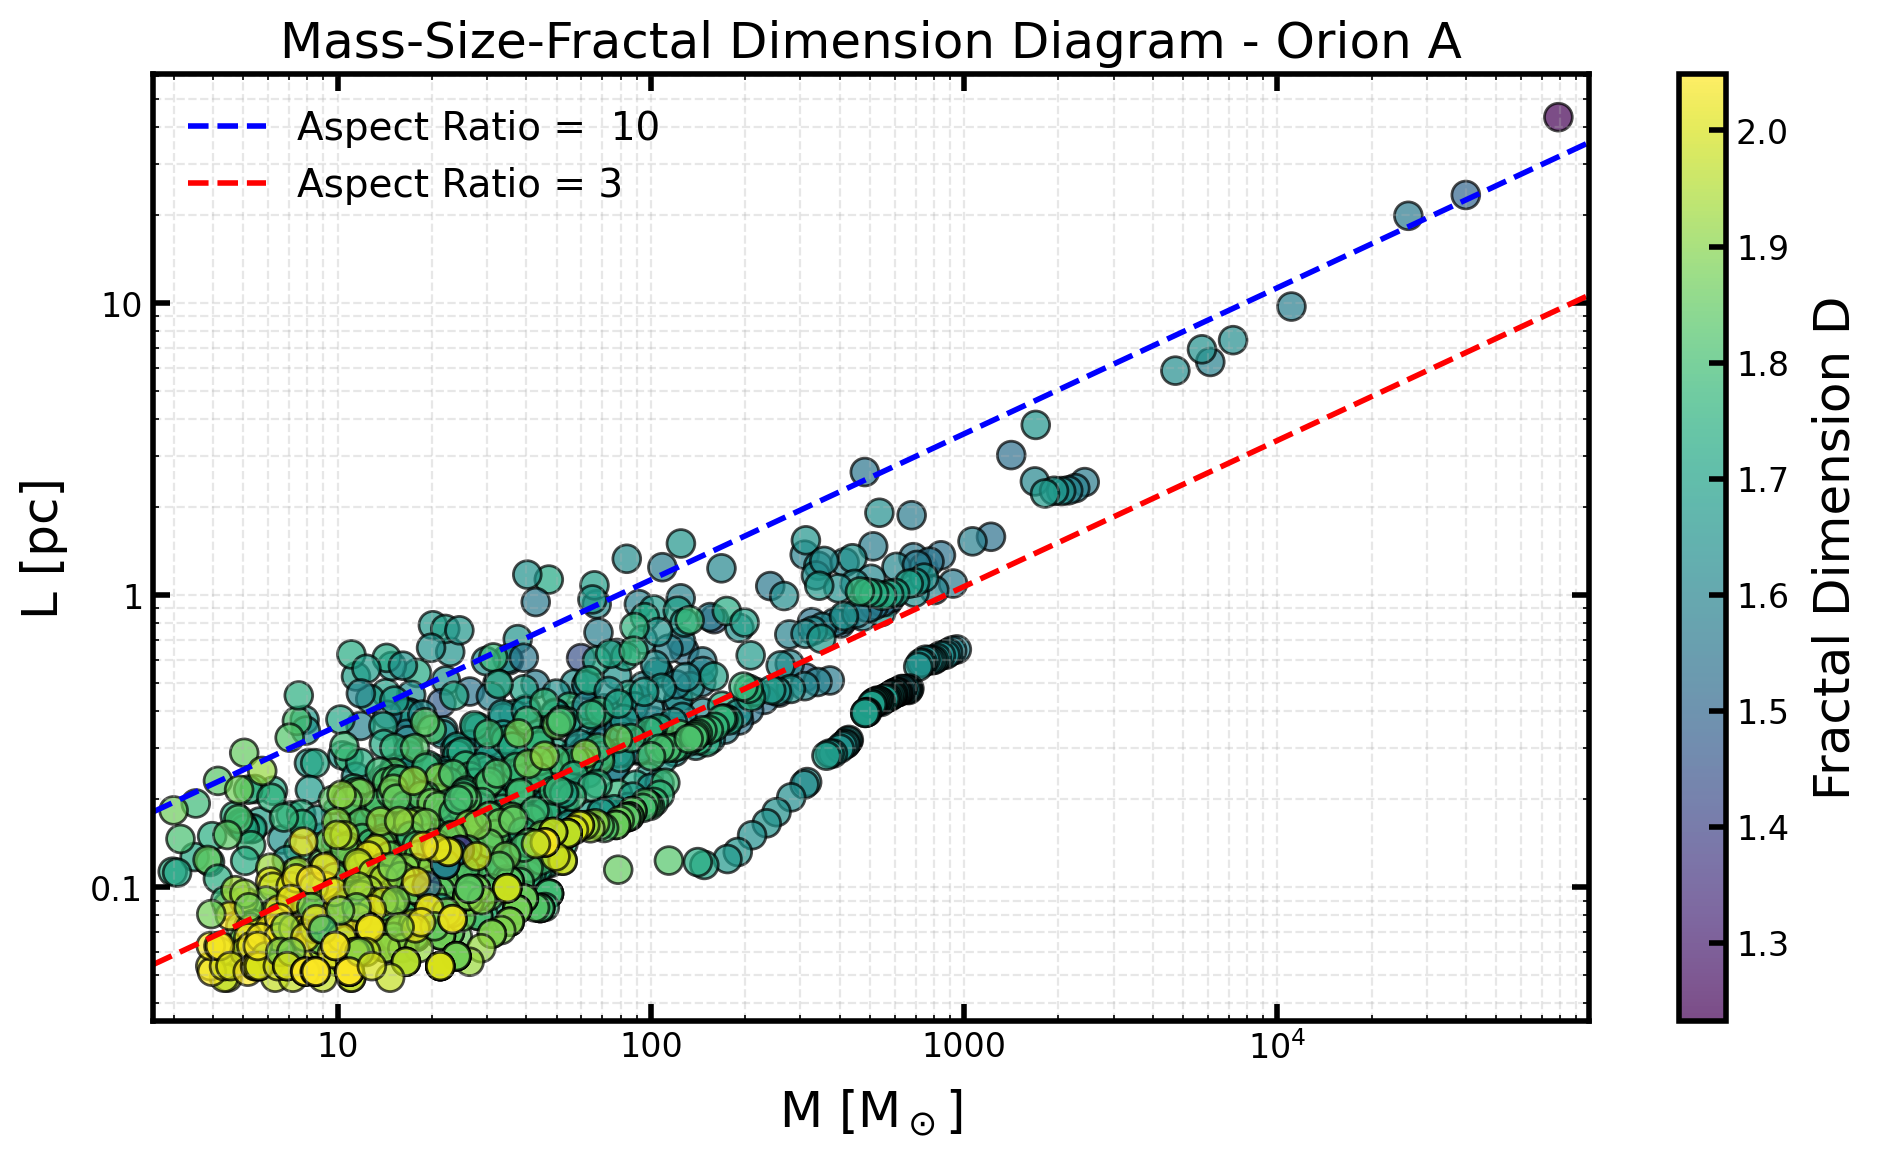
\includegraphics[width=0.75\textwidth]{figures/MSD_Orion_A.png}
    \caption{MSD plane for Orion A. Expected scaling for filamentary and spherical structures are plotted as well.}
    \label{fig:MSD_orion_A}
\end{figure}

\begin{figure}[t]
    \centering
    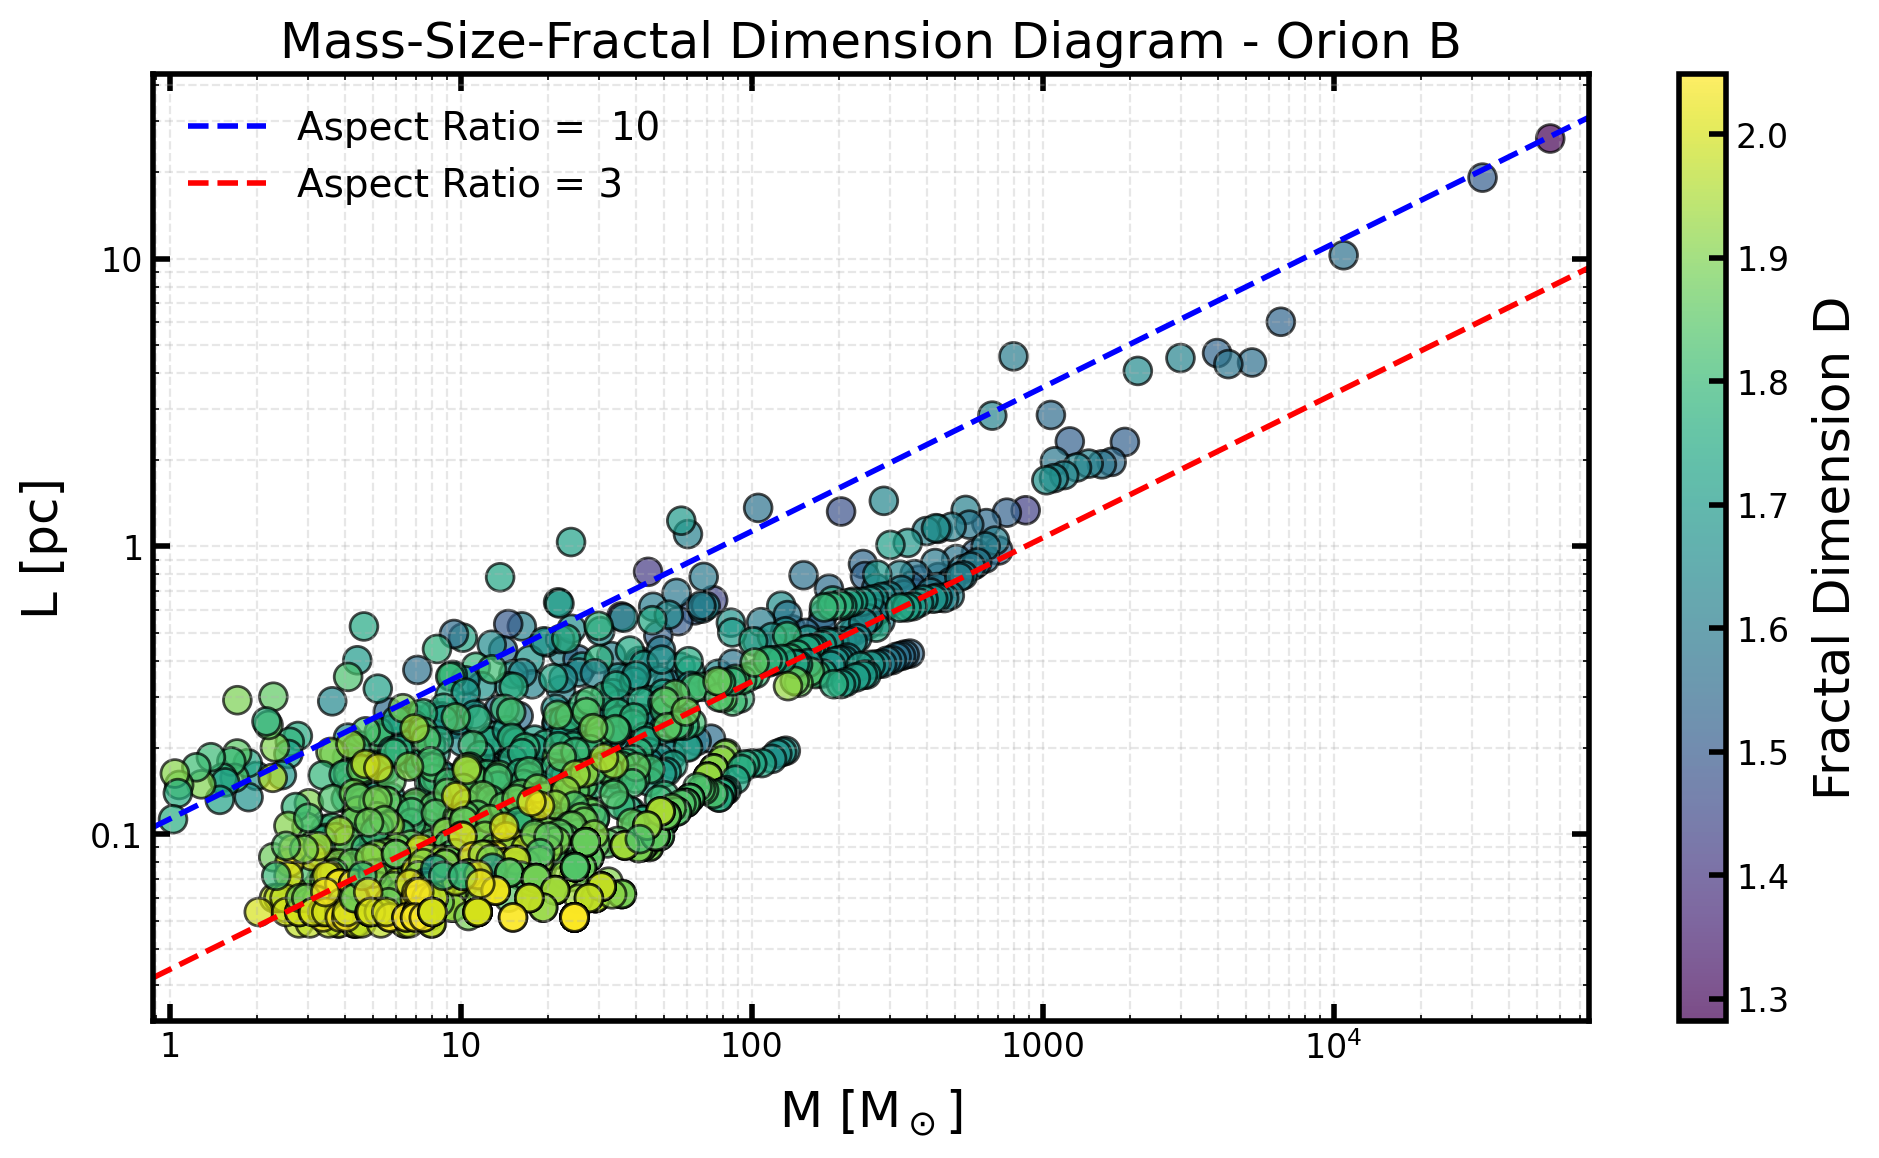
\includegraphics[width=0.75\textwidth]{figures/MSD_Orion_B.png}
    \caption{MSD plane for Orion B. Expected scaling for filamentary and spherical structures are plotted as well.}
    \label{fig:MSD_orion_B}
\end{figure}

\begin{figure}[t]
    \centering
    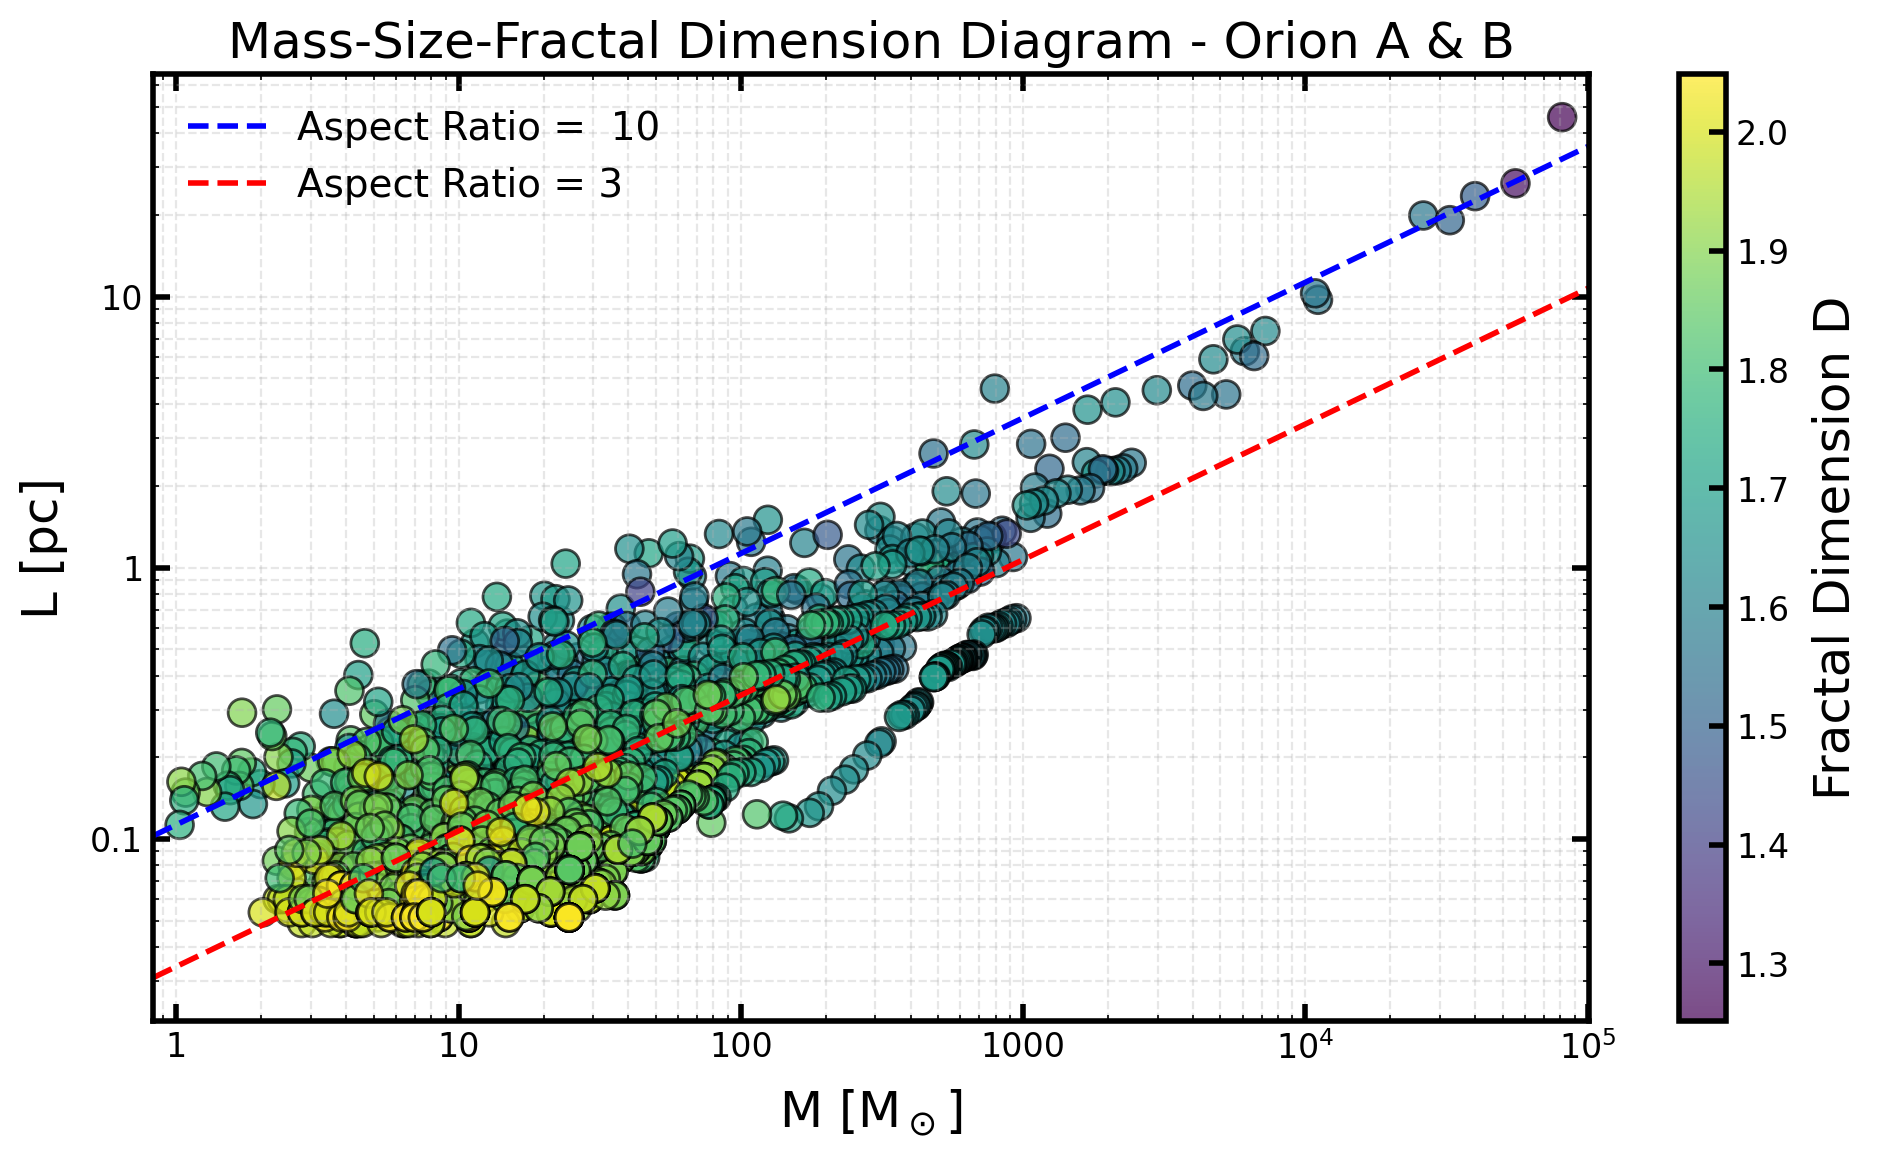
\includegraphics[width=0.75\textwidth]{figures/MSD_Orion_A_B.png}
    \caption{MSD plane for Orion A and B combined. Expected scaling for filamentary and spherical structures are plotted as well. The color bar is based on the entirety of the combined dataset.}
    \label{fig:MSD_orion_A_B}
\end{figure}

Using the information obtained so fra, we can connect this to the mask and location of the structures, and one can create a phsical map of the local fractal dimension. This is specifically done by assigning to each of the pixel within the mask the value of the corresponding fractal dimension, and then averaging when more structures share common areas.
Since this is an averaging process, the higher values are a bit lower than what was presented in the previous pictures. However, this further confirms and shows the trend observed so far.
Orion A and Orion B.

\begin{figure}[t]
    \centering
    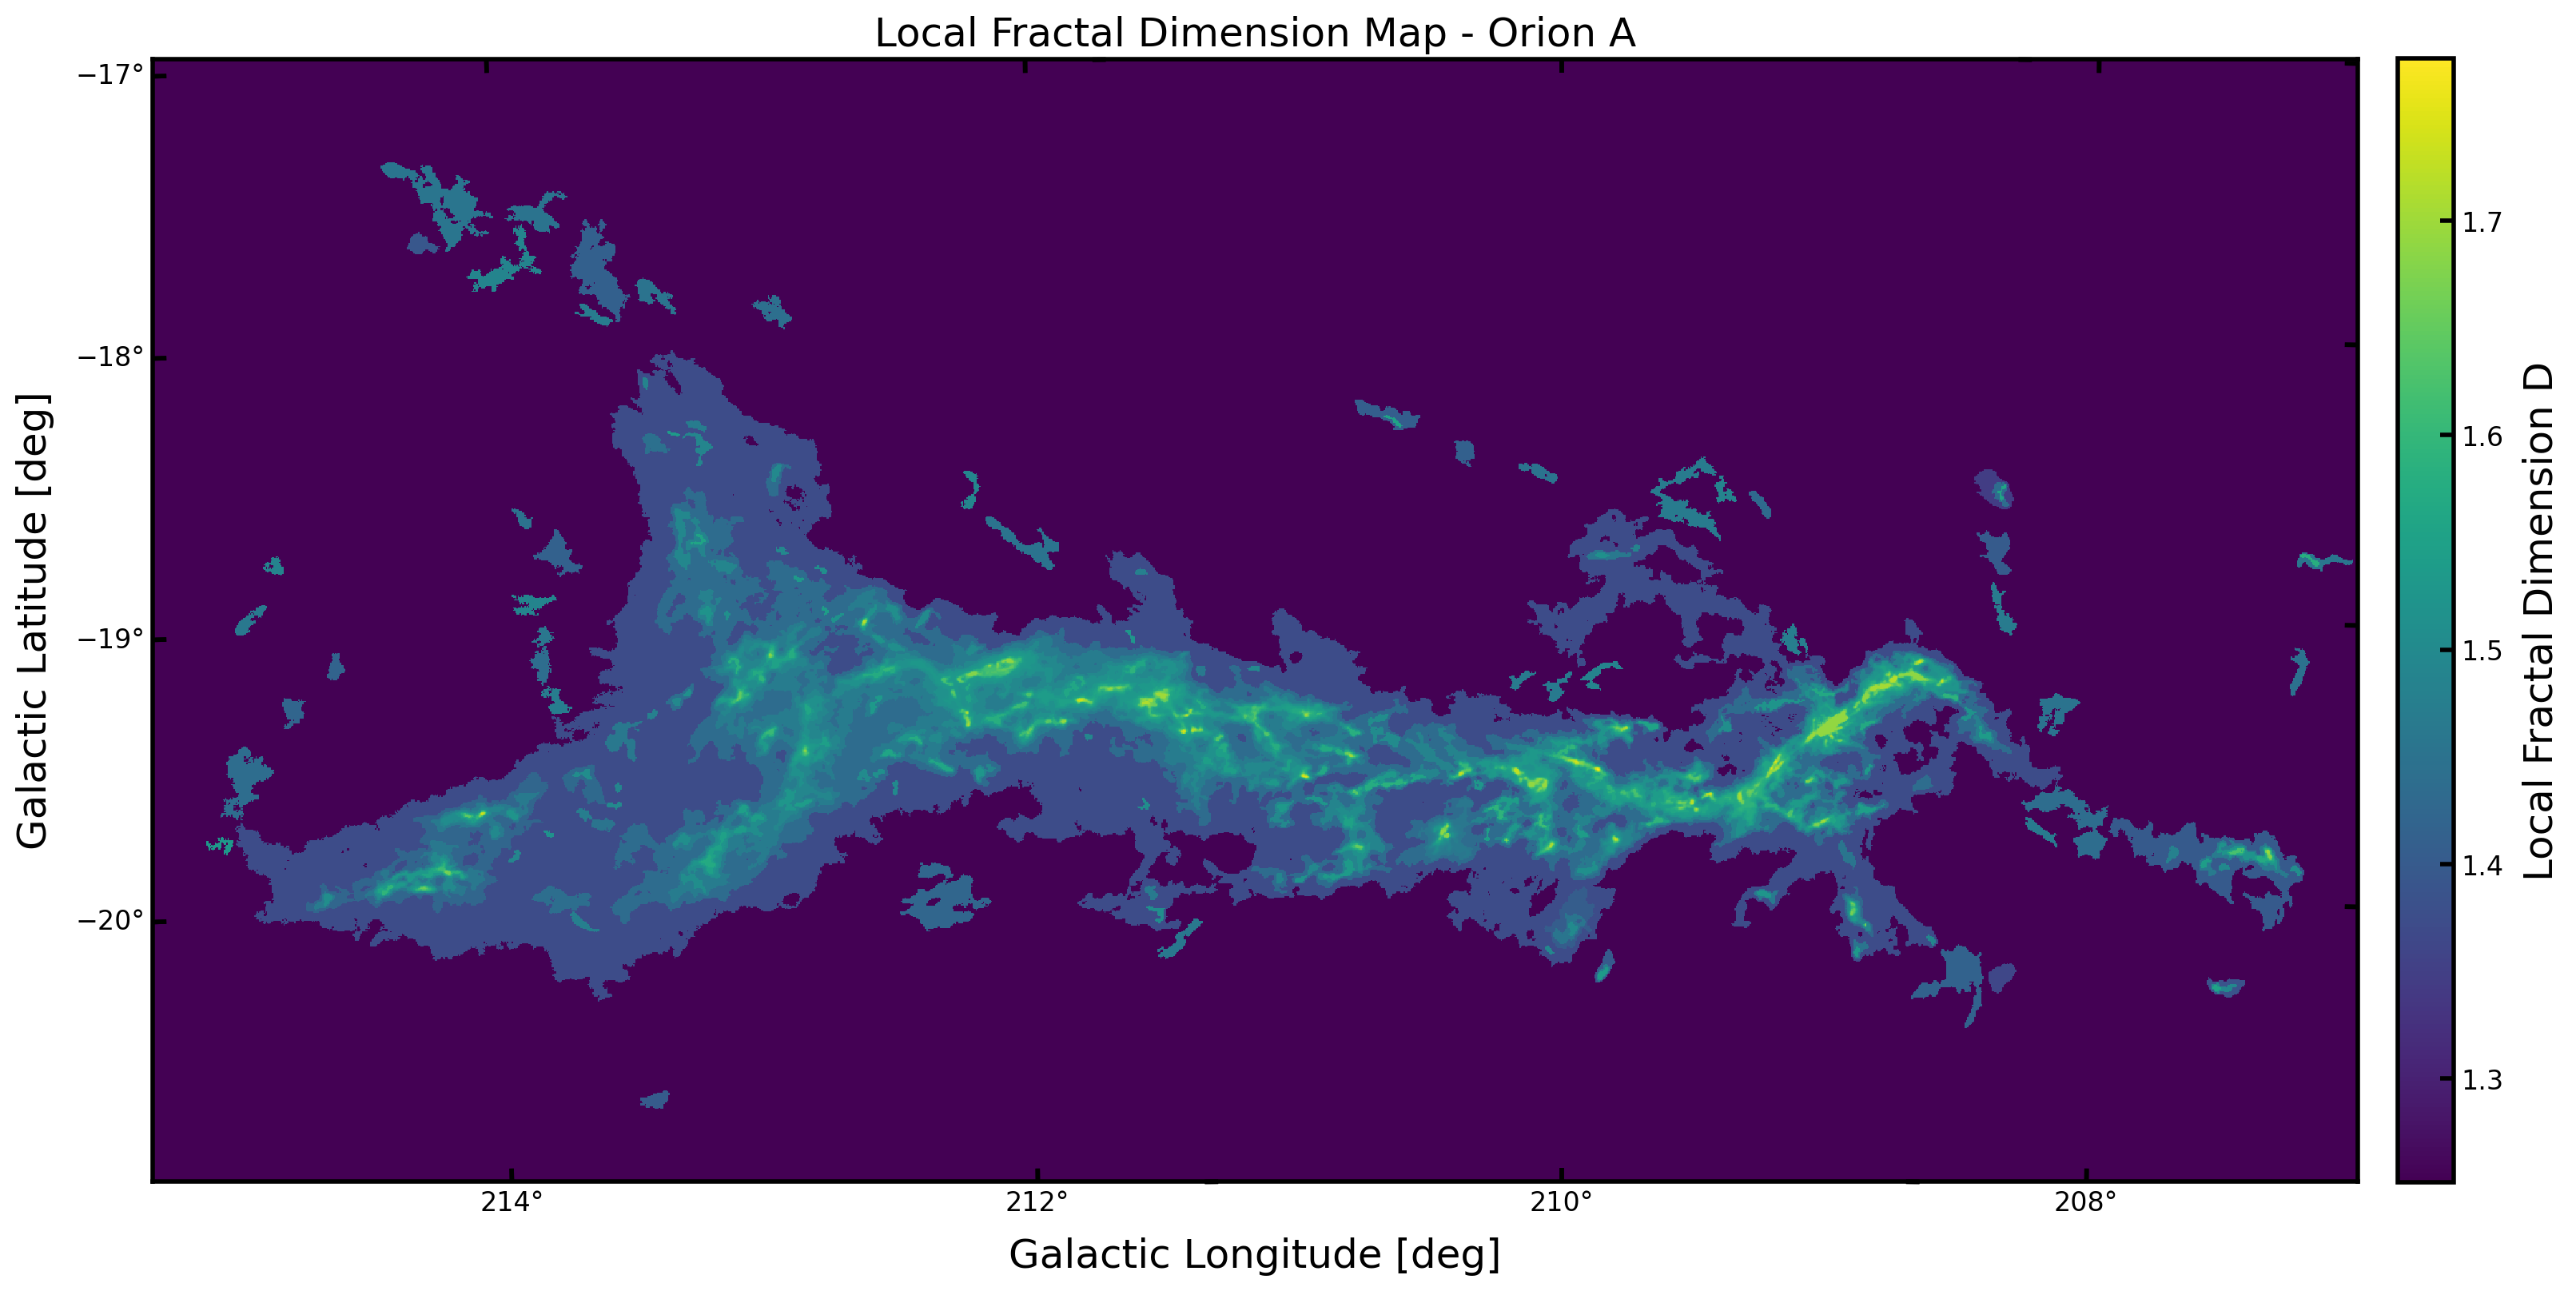
\includegraphics[width=0.75\textwidth]{figures/local_fractal_dimension_map_Orion_A.png}
    \caption{Physical map of the local fractal dimension for Orion A. NaN values are set to the lowest found value of the fractal dimension.}
    \label{fig:local_A_map}
\end{figure}

% to-do:
% zoom in (cut the right side)
% remove the straight lines 
\begin{figure}[t]
    \centering
    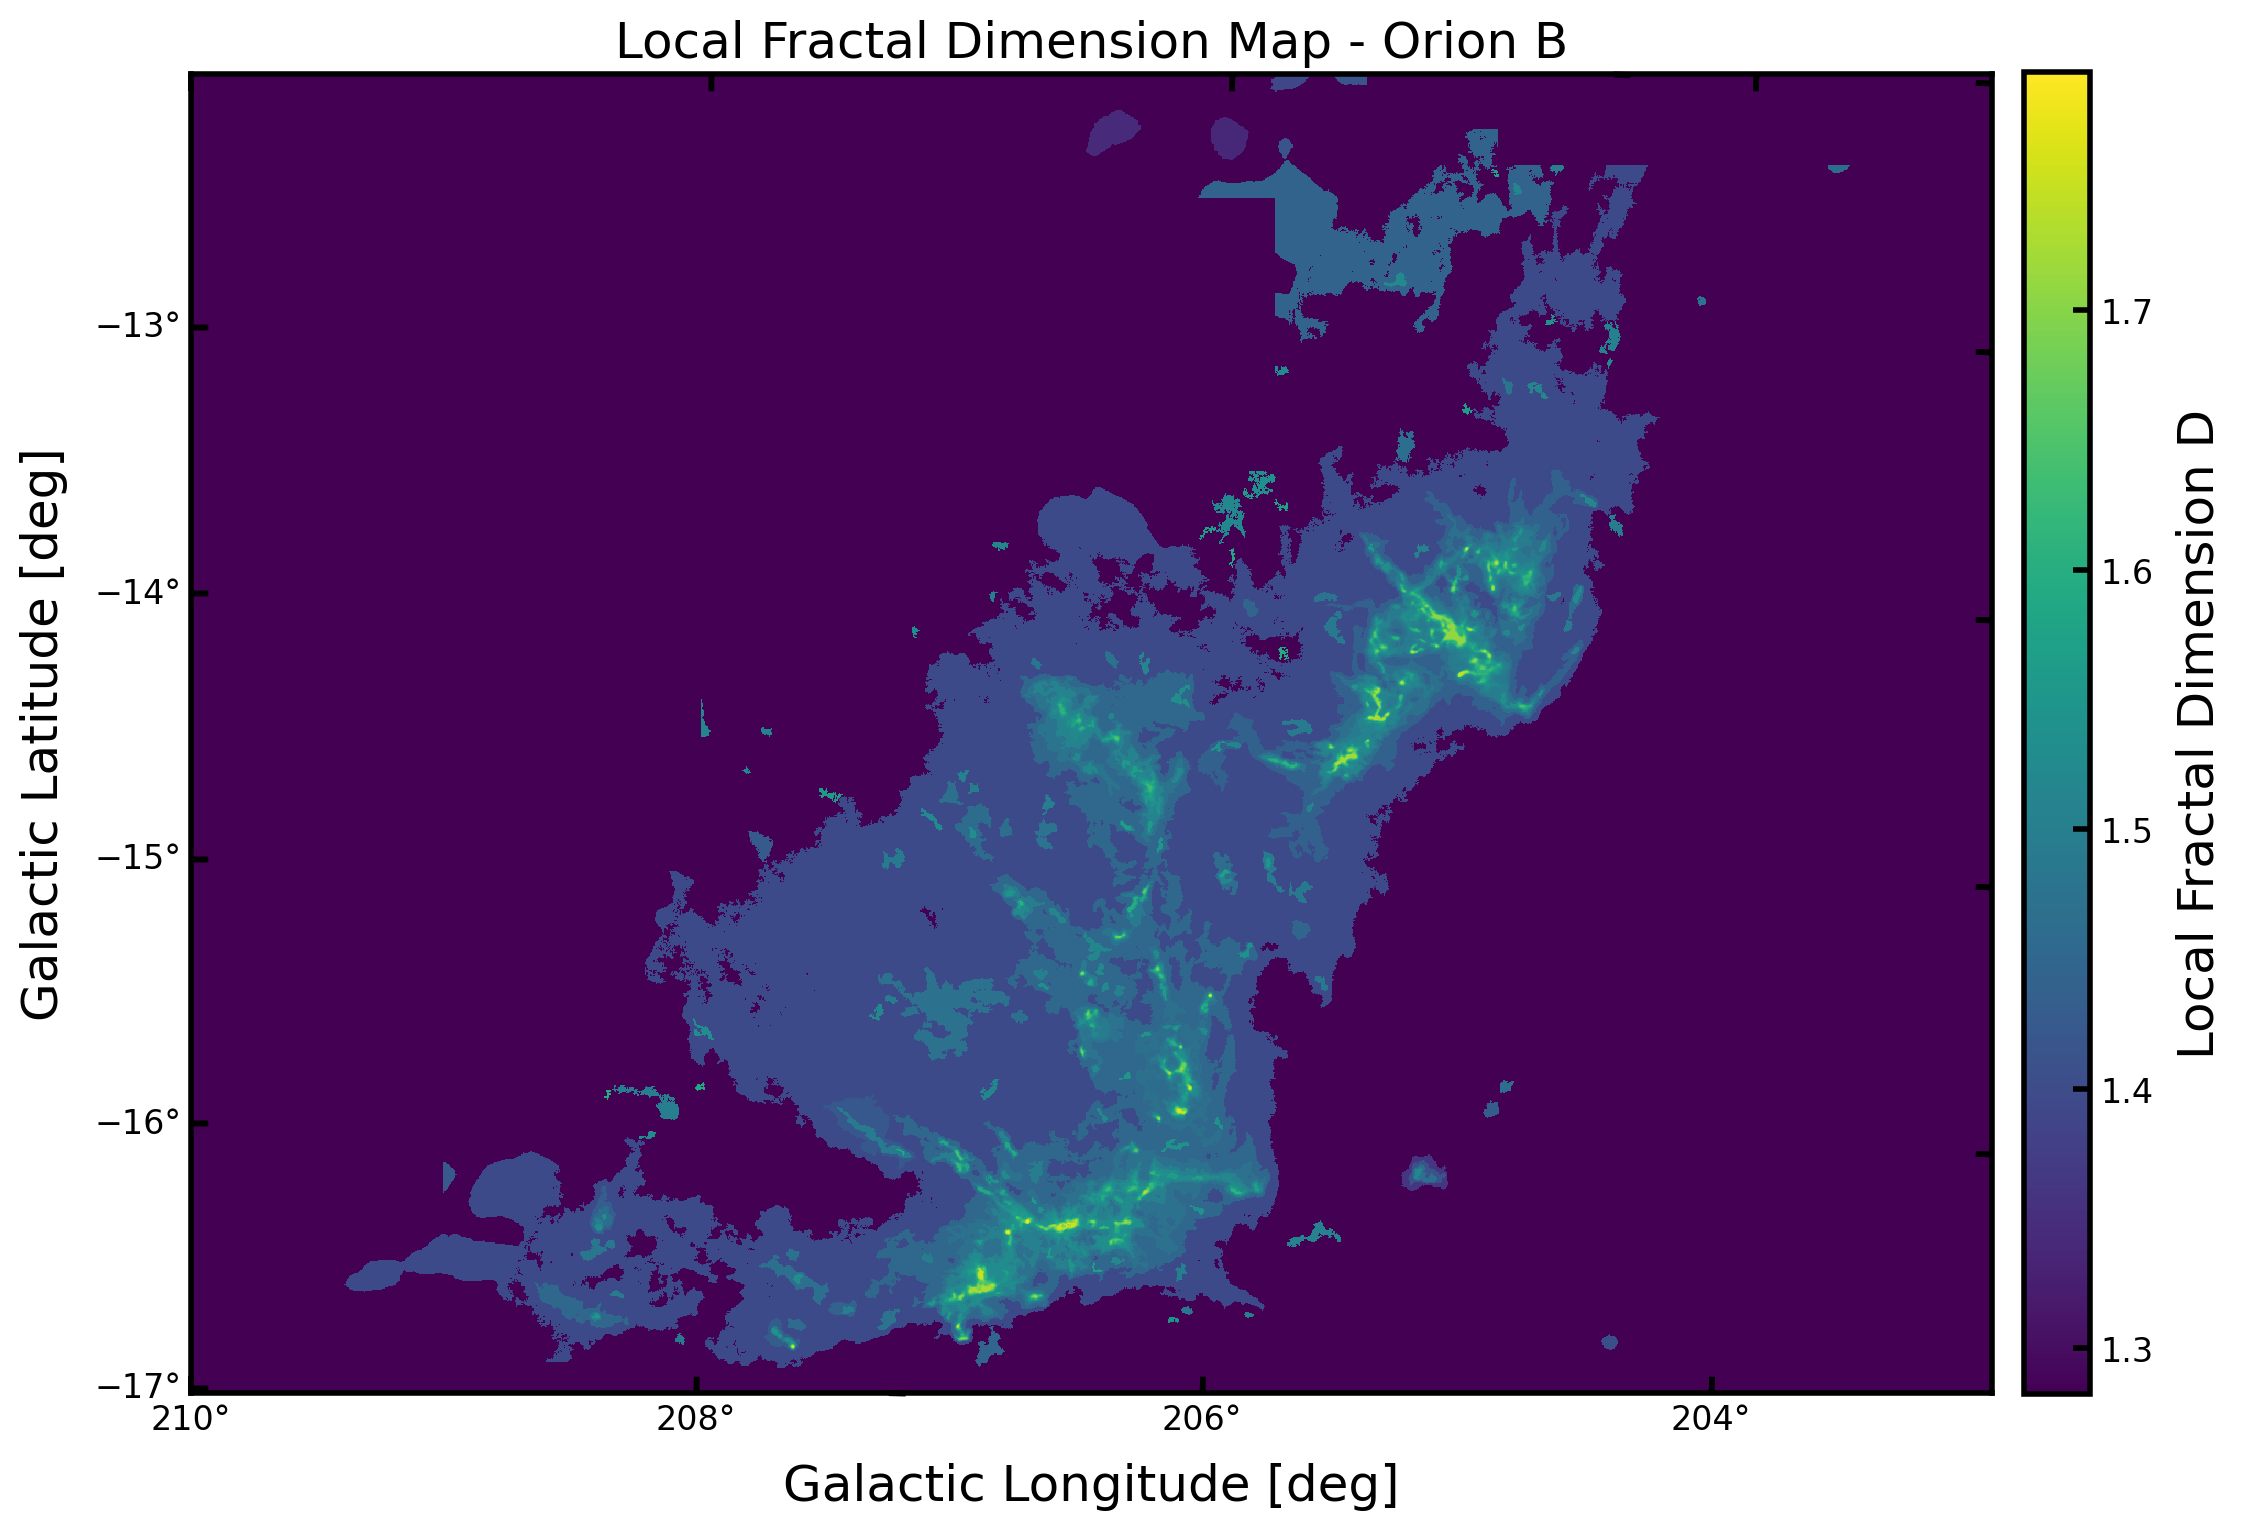
\includegraphics[width=0.75\textwidth]{figures/local_fractal_dimension_map_Orion_B.png}
    \caption{Physical map of the local fractal dimension for Orion B. NaN values are set to the lowest found value of the fractal dimension.}
    \label{fig:local_B_map}
\end{figure}

The MSD plane can also be visualized in 3D. Check the website for interactivity \href{https://simonesped.github.io/MSD_Viz/}{MSD Visualizer}.

Dendrograms allow to track the break-down of structures, hence this information can be plotted as well by drawing lines between parent and child structures. 
This can be seen in Figures \ref{fig:MSD_orion_A_lines} and \ref{fig:MSD_orion_B_lines} for Orion A and B.

% to-do
% likely to redo, very messy
\begin{figure}[t]
    \centering
    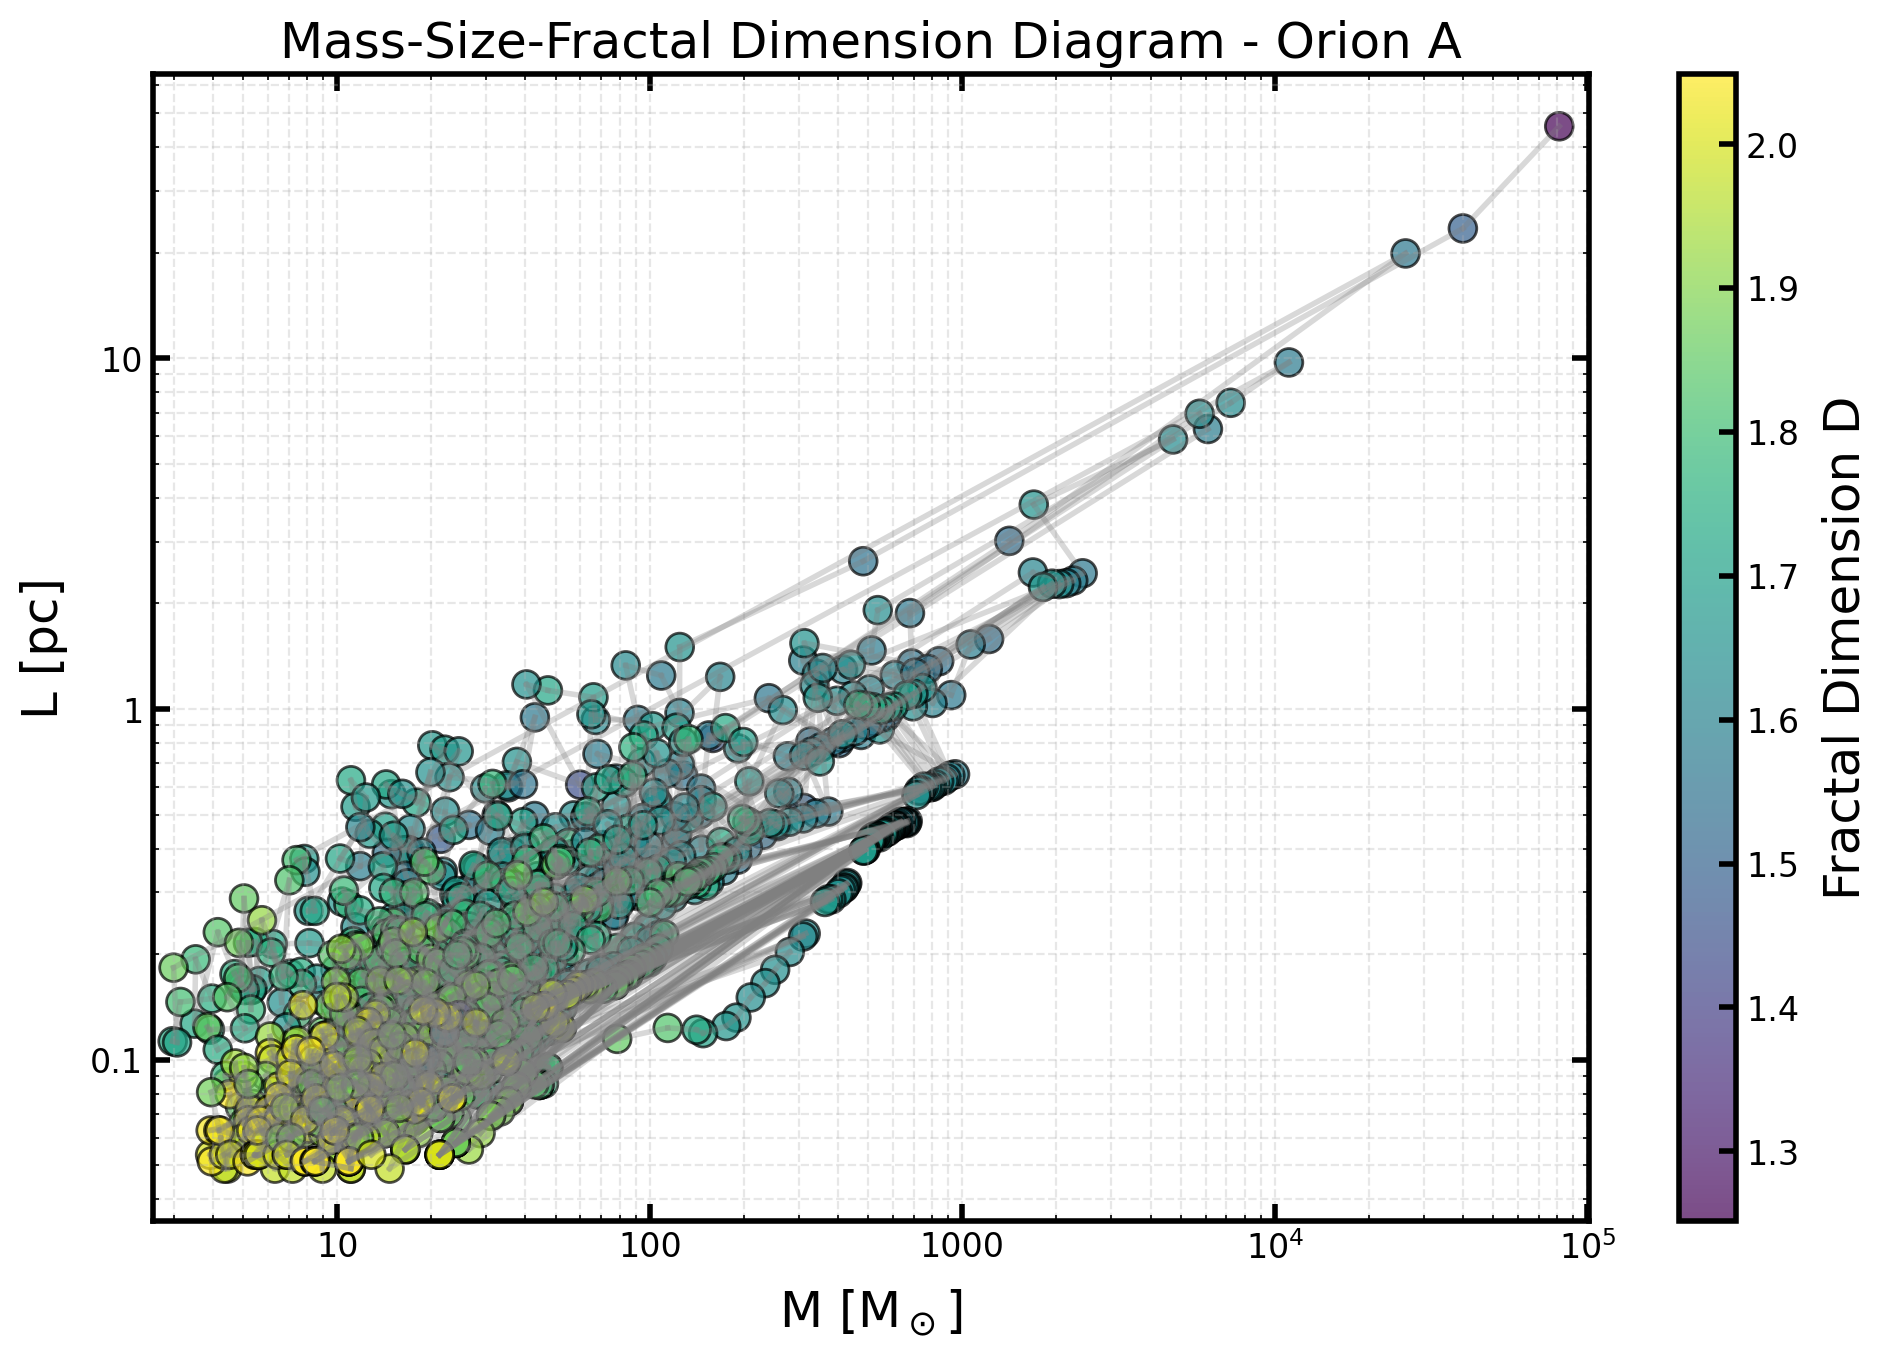
\includegraphics[width=0.75\textwidth]{figures/MSD_Orion_A_with_lines.png}
    \caption{MSD plane for Orion A with lines connecting dendrogram parents and children.}
    \label{fig:MSD_orion_A_lines}
\end{figure}

\begin{figure}[t]
    \centering
    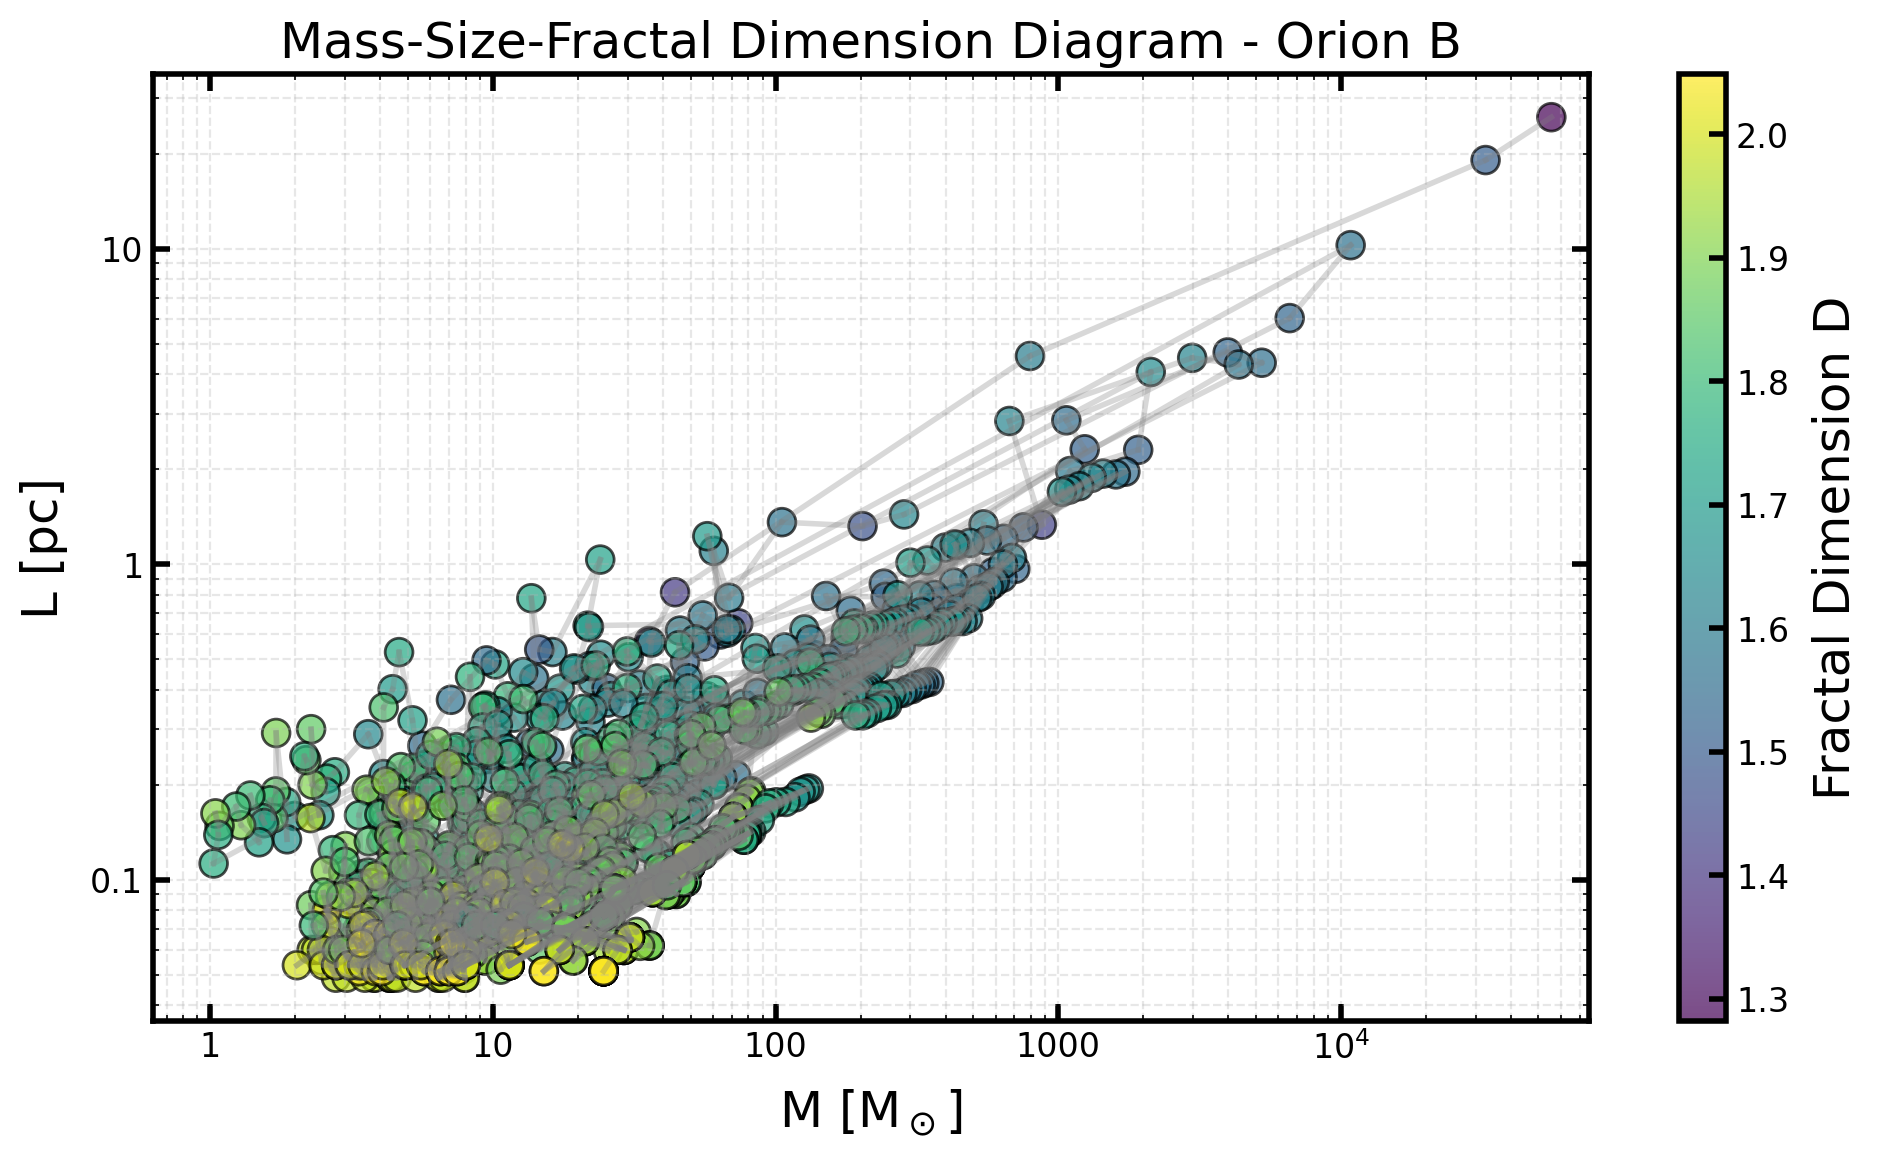
\includegraphics[width=0.75\textwidth]{figures/MSD_Orion_B_with_lines.png}
    \caption{MSD plane for Orion B with lines connecting dendrogram parents and children.}
    \label{fig:MSD_orion_B_lines}
\end{figure}

% YSOs (which stage of evolution are to be considered?)
\section{Star Formation}

Higher density regions are expected to be more prone to star formation, hence we can use the local fractal dimension to estimate the likelihood of star formation in a given region. 
This is done by comparing the local fractal dimension with the YSO density map, which is derived by smoothing out the distribution of YSOs in the region. 
The density map for Orion A is for example shown in Figure \ref{fig:YSOs_density_Map_A}.  Orion B looks fairly similar.

\begin{figure}[t]
    \centering
    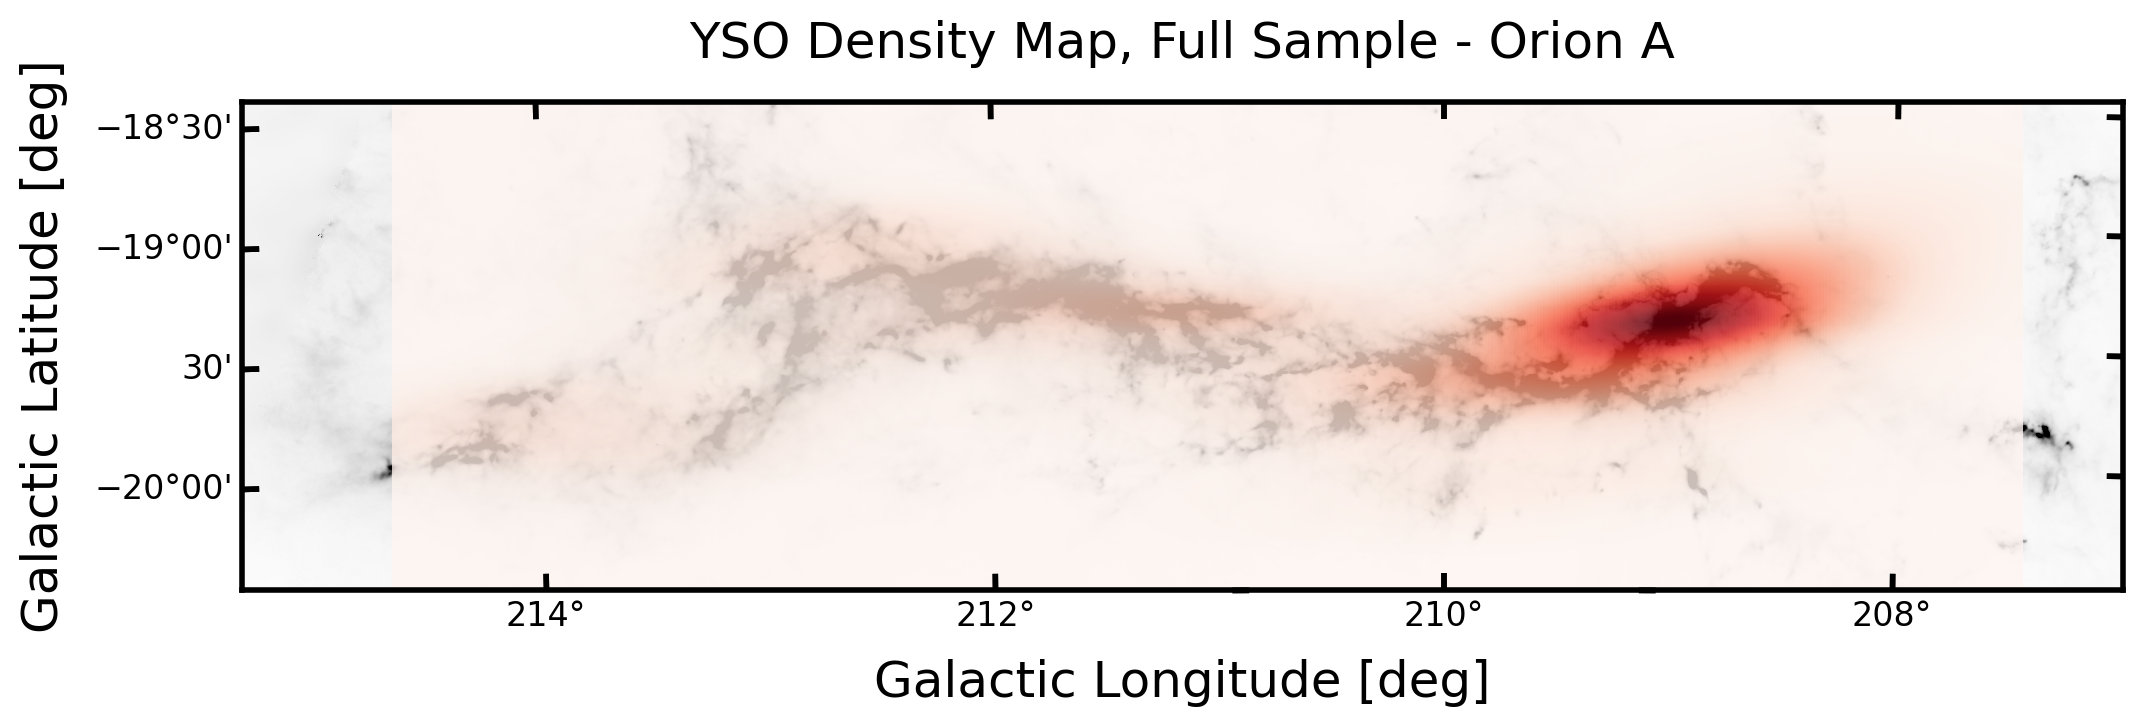
\includegraphics[width=0.75\textwidth]{figures/YSOs_density_Orion_A.png}
    \caption{YSO density map of Orion A overlaid on top of the column density one. The YSO density coverage is limited by the extent of the coordinates of the YSOs, hence not everything is covered.}
    \label{fig:YSOs_density_Map_A}
\end{figure}

The bitwise correlation between the two maps for Orion A and is:

Pearson correlation: 0.286 
Spearman correlation: 0.393 

and Orion B:

Pearson correlation: 0.399
Spearman correlation: 0.340

% maybe not a lot of pictures here: TBD
\section{Simulations and Uncertainties}

\subsection{Simulations on Global Properties}

\subsubsection{On the Global Fractal Dimension}
Interpretation of Global Fractal Dimension
Scale-free GRF vs GRF with Scale
Resolution Effects

\subsection{Simulations on Local Properties}

% maybe a diagram? not entirely necessary imo
\subsubsection{On the Euler Characteristic}
Simulations were also carried out to have a better feeling of what to expect from the Euler Characteristic when applied to real cases. The main subject of these simulations were Gaussian Random Fields, with the expectation of a symmetric behaviour. That was indeed the case, highlighting a maximum in connectivity where the peak is, and both before and after a decrease in such in a way that resembles a Gaussian Bell.

\subsubsection{On the Local Fractal Dimension}
Validity Stuff + Interpretation
Resolution Effects

\subsection{Error estimates}

The uncertainties on the perimeter and area measurements, estimated using the simulation procedures described above, are on average approximately 1.60\% for each quantity. These uncertainties arise primarily from pixelation effects and resolution limitations in the column density maps.  

An example of the resulting error distributions from a representative simulation run is shown in Figure~\ref{fig:uncertainties}. The narrow spread around the mean confirms that the estimates are robust and systematic errors remain small compared to the dynamic range of the measurements.

\begin{figure}[t]
    \centering
    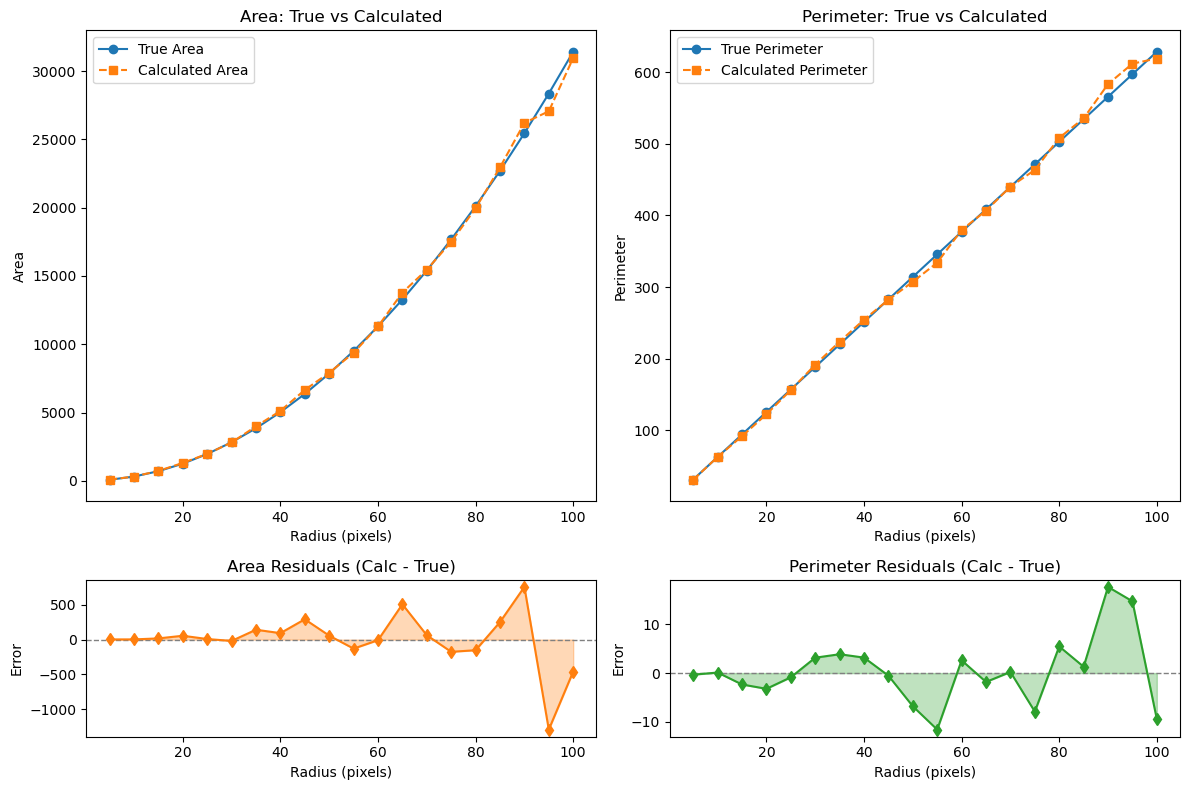
\includegraphics[width=0.75\textwidth]{figures/perimeter_area_uncertainties.png}
    \caption{Example of the uncertainty distributions in the measurements of perimeter and area from simulated structures (arbitrary units).}
    \label{fig:uncertainties}
\end{figure}

\subsection{Comparison with alternative methods}

A clear anti-correlation is observed when comparing results with the box-counting method, both for the global and local estimates of the fractal dimension. This highlights an interesting scaling property that should be taken into account when comparing studies that employ different techniques for quantifying fractal characteristics.
